\documentclass{article}[a4paper, oneside,11pt]
\usepackage[utf8]{inputenc}
\usepackage[a4paper, total={6in, 10in}]{geometry}
\usepackage{graphicx}
\usepackage{float}
\usepackage{amsmath}
\usepackage[italian]{babel}
\usepackage{titlesec}
\usepackage{multirow}

\title{SIMULAZIONE NUMERICA DELLA SERIE DI FOURIER}
\author{JACOPO MARTELLOTTO\\ERIK EJRNAES}
\date{Dicembre 2023 - Gennaio 2024}

\begin{document}
\maketitle

\section{Ricostruzione di forme d'onda}
    \subsection{Onda quadra}
    L'onda quadra può essere ricostruita numericamente tramite l'espansione in serie di Fourier:
    \begin{align}
        f(t) = \frac{f_0}{2} + \sum_{k=1}^{n} \left(b_k \cos{\omega_k t} + c_k \sin{\omega_k t} \right) 
        \label{Serie di Fourier}
    \end{align}
    Dove $n$ determina il troncamento della serie. Nel nostro caso, poiché l'onda che abbiamo approssimato è dispari $b_k = 0$, mentre per i $c_k$ per l'onda quadra vale:
    \begin{align*}
        c_k &= 0 \qquad k \text{ pari}\\
        c_k &= \frac{2}{k\pi} \quad k \text{ dispari}
    \end{align*}
    Abbiamo ricostruito numericamente l'onda quadra per vari valori del troncamento $n$ e per vari possibili intervalli di campionamento (da $-t_{max}$ a $t_{max}$):
        \begin{figure}[H]
            \centering
            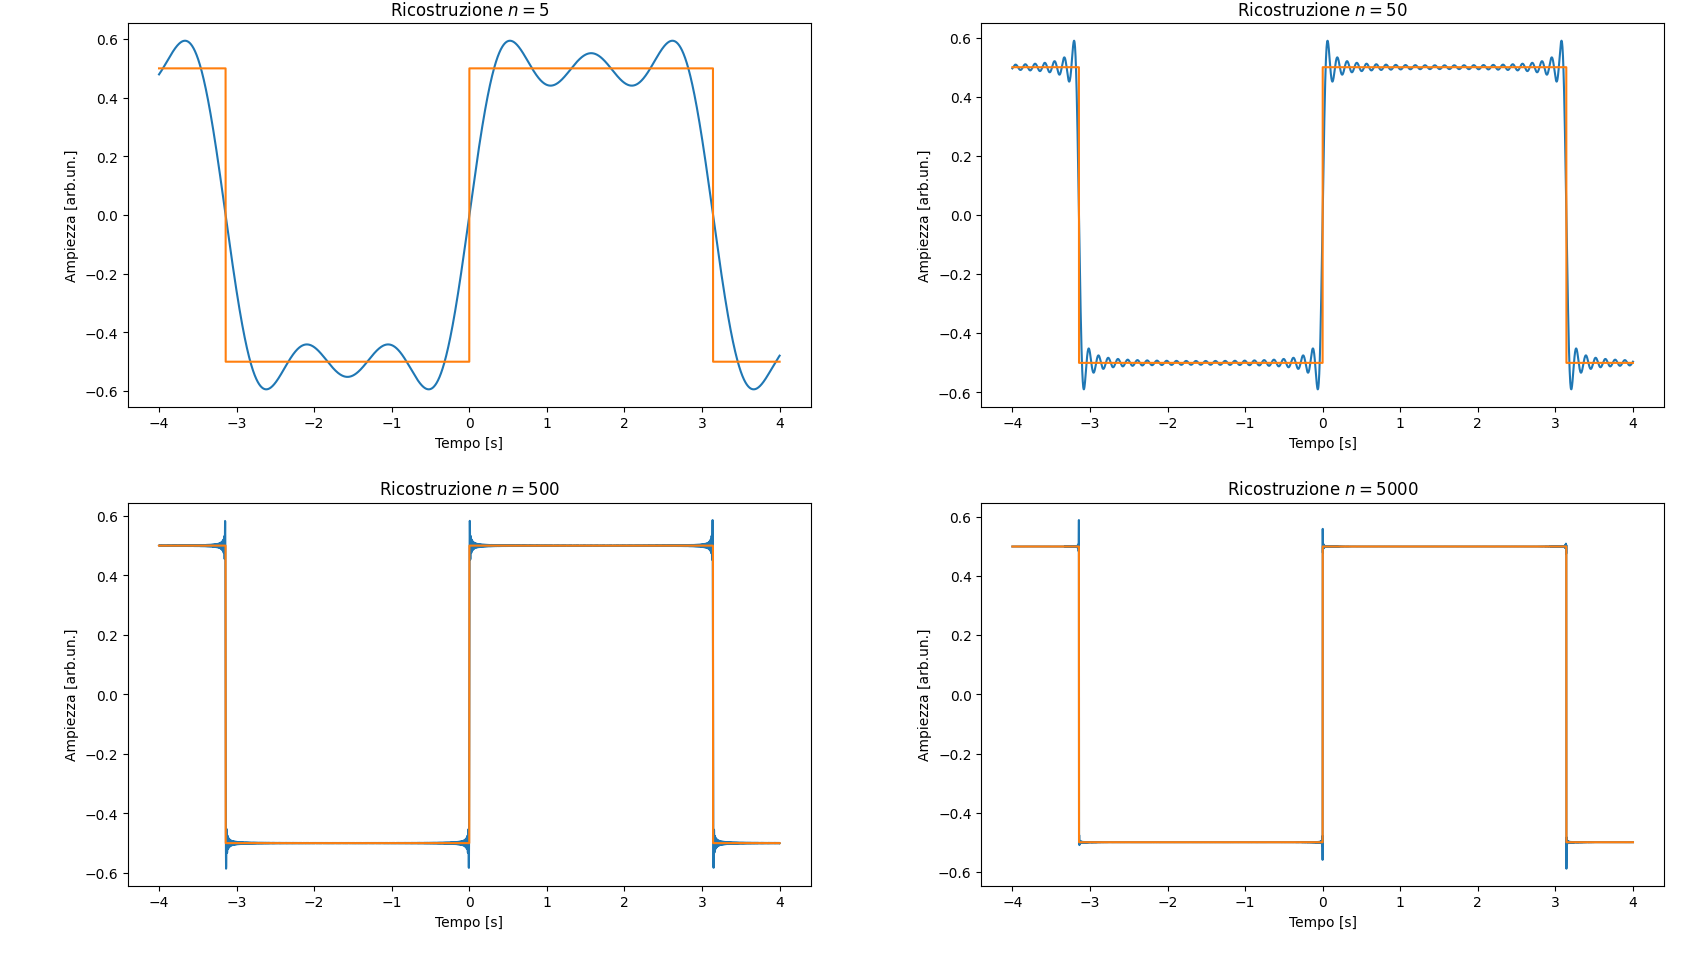
\includegraphics[width=0.9\textwidth]{img/Ricostruzione_onda_quadra_troncamento.png}
            \caption{Ricostruzioni al variare di $n$, per $t_{max}=4$ s.}
            \label{Fig_OQT}
        \end{figure}
        \begin{figure}[H]
            \centering
            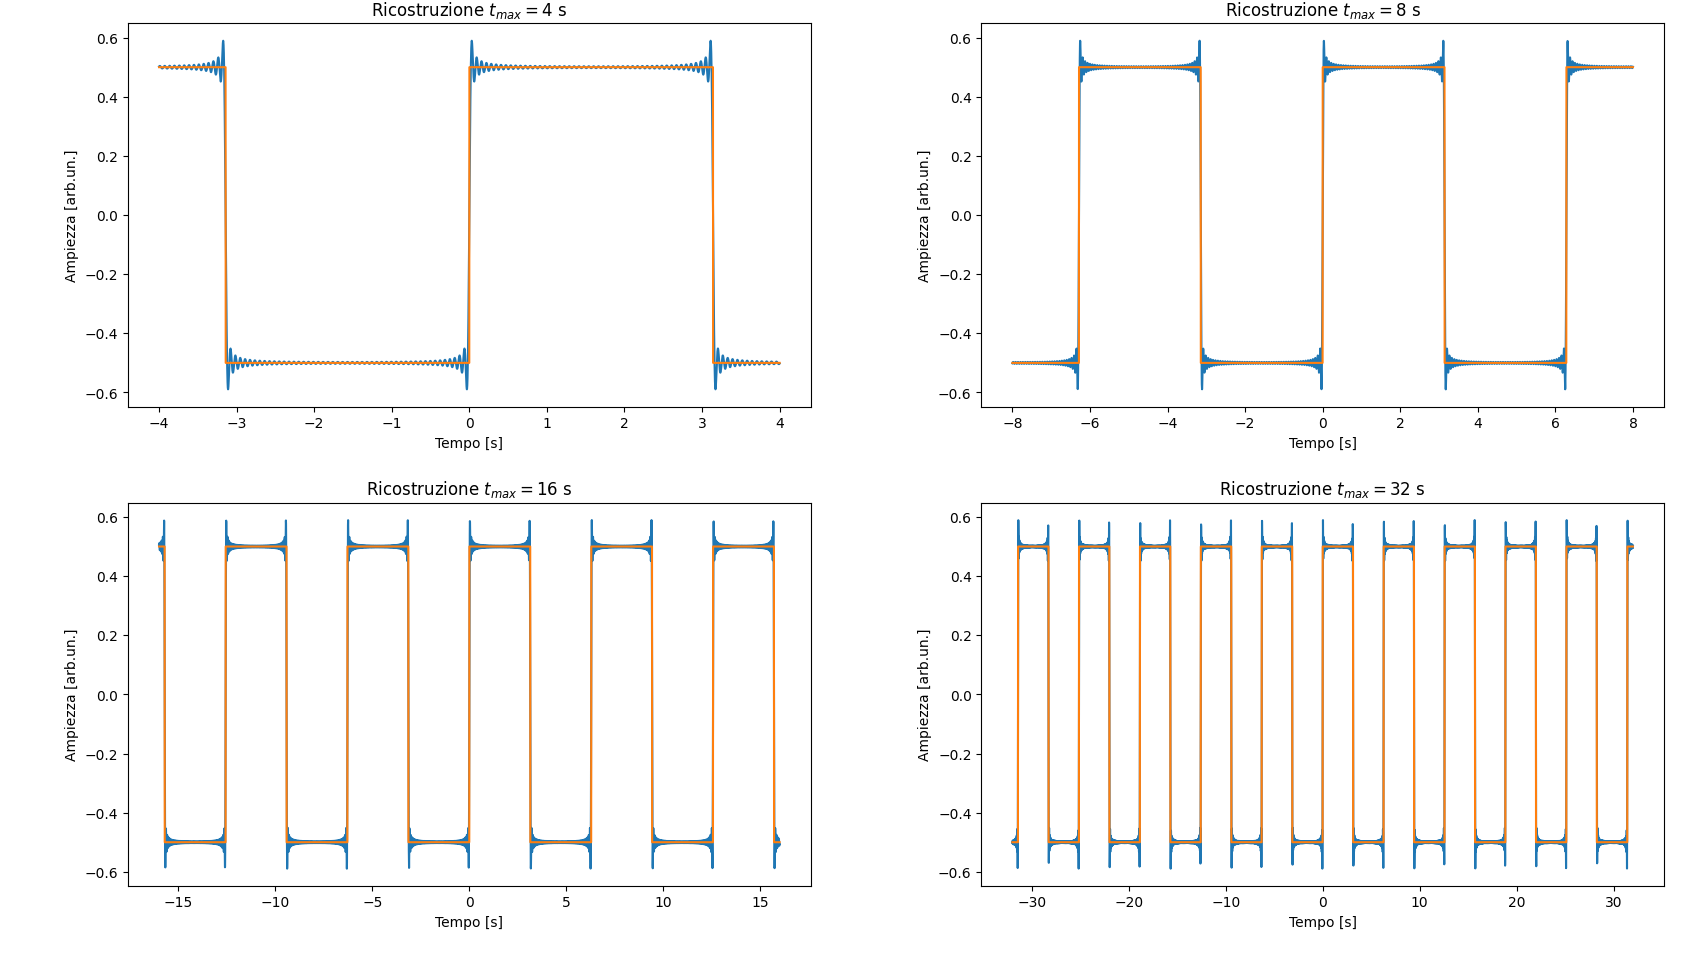
\includegraphics[width=0.9\textwidth]{img/Ricostruzione_onda_quadra_campionamento.png}
            \caption{Ricostruzioni al variare di $t_{max}$, per $n=10$.}
            \label{Fig_OQC}
        \end{figure}
    \noindent Dai grafici possiamo notare delle "sovra elongazioni" intorno ai salti dell'onda quadra. Questo è dovuto al fatto che approssimiamo la forma d'onda, che ha derivata teoricamente infinita in quei punti, con seni e coseni che, invece, hanno derivata finita. Questo effetto è noto come \textit{fenomeno di Gibbs}.\\
    Inoltre, per intervalli di campionamento ampi, possiamo notare come apparentemente la forma d'onda ricostruita non sia perfettamente periodica; in particolare i picchi del fenomeno di Gibbs appaiono più o meno alti nelle varie oscillazioni. Questo potrebbe apparire strano, dato che la funzione ricostruita è una somma di funzioni periodiche e quindi dovrebbe essere essa stessa periodica. In realtà quello che succede qui è dovuto al fatto che per rappresentare la funzione su un grafico abbiamo dovuto fare un \textit{sampling} a punti spaziati diversamente dai periodi dei termini dell'espansione. Si potrebbe dire che questo è la versione unidimensionale dell'\textit{effetto Moiré}.\\
    
    
    \subsection{Onda triangolare}
    Per l'onda triangolare, invece, nell'espressione:
    \begin{align*}
        g(t) = \frac{g_0}{2} + \sum_{k=1}^{n} \left(b_k \cos{\omega_k t} + c_k \sin{\omega_k t} \right) 
    \end{align*}
    poiché l'onda stavolta è pari $c_k = 0$, mentre per i $b_k$, possiamo distinguere i seguenti casi: 
    \begin{align*}
        b_k &= 0 \qquad \qquad k \text{ pari}\\
        b_k &= \left(\frac{2}{k \pi}\right)^2 \quad k \text{ dispari}
    \end{align*}
    
    \noindent Come per l'onda quadra, abbiamo ricostruito numericamente l'onda triangolare per vari valori del troncamento $n$ e per vari possibili intervalli di campionamento (da $-t_{max}$ a $t_{max}$). Poiché l'onda triangolare è meglio approssimata dalla serie troncata di quella quadra a parità di $n$, abbiamo anche provato valori di $n$ più piccoli.
        \begin{figure}[H]
            \centering
            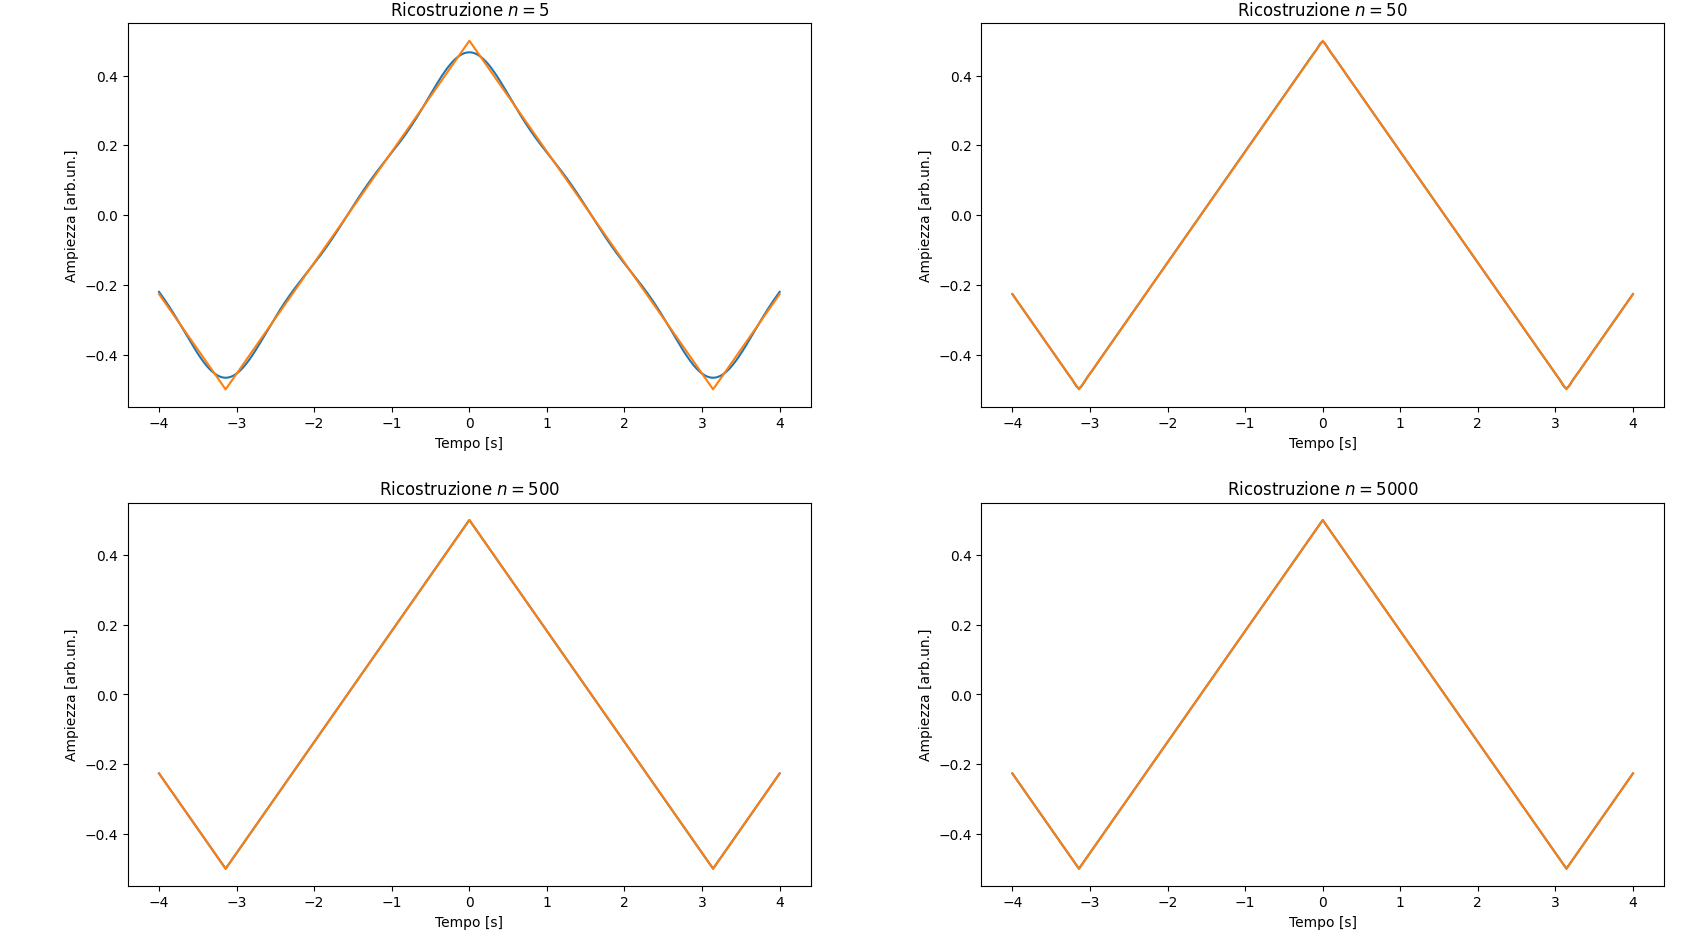
\includegraphics[width=0.84\textwidth]{img/Ricostruzione_onda_triangolare_troncamento.png}
            \caption{Ricostruzioni al variare di $n$, per $t_{max}=4$ s.}
            \label{Fig_OTT}
        \end{figure}\begin{figure}[H]
            \centering
            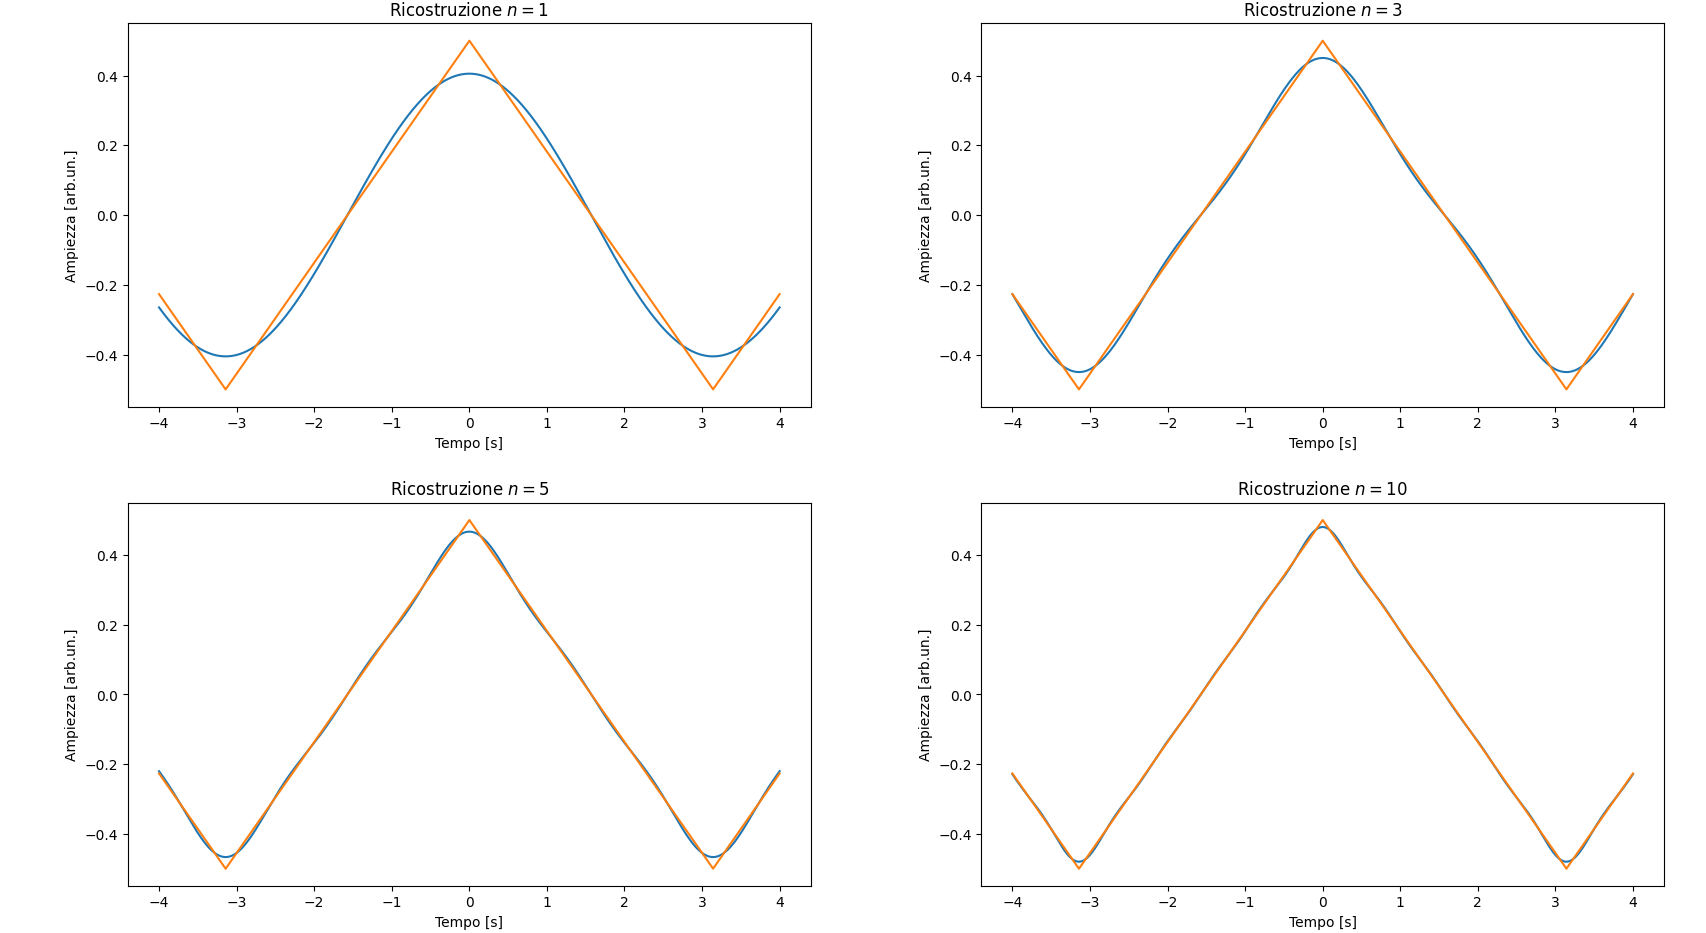
\includegraphics[width=0.84\textwidth]{img/Ricostruzione_onda_triangolare_troncamento_basso.png}
            \caption{Altre ricostruzioni al variare di $n$, per $t_{max}=4$ s.}
            \label{Fig_OTTB}
        \end{figure}
        \begin{figure}[H]
            \centering
            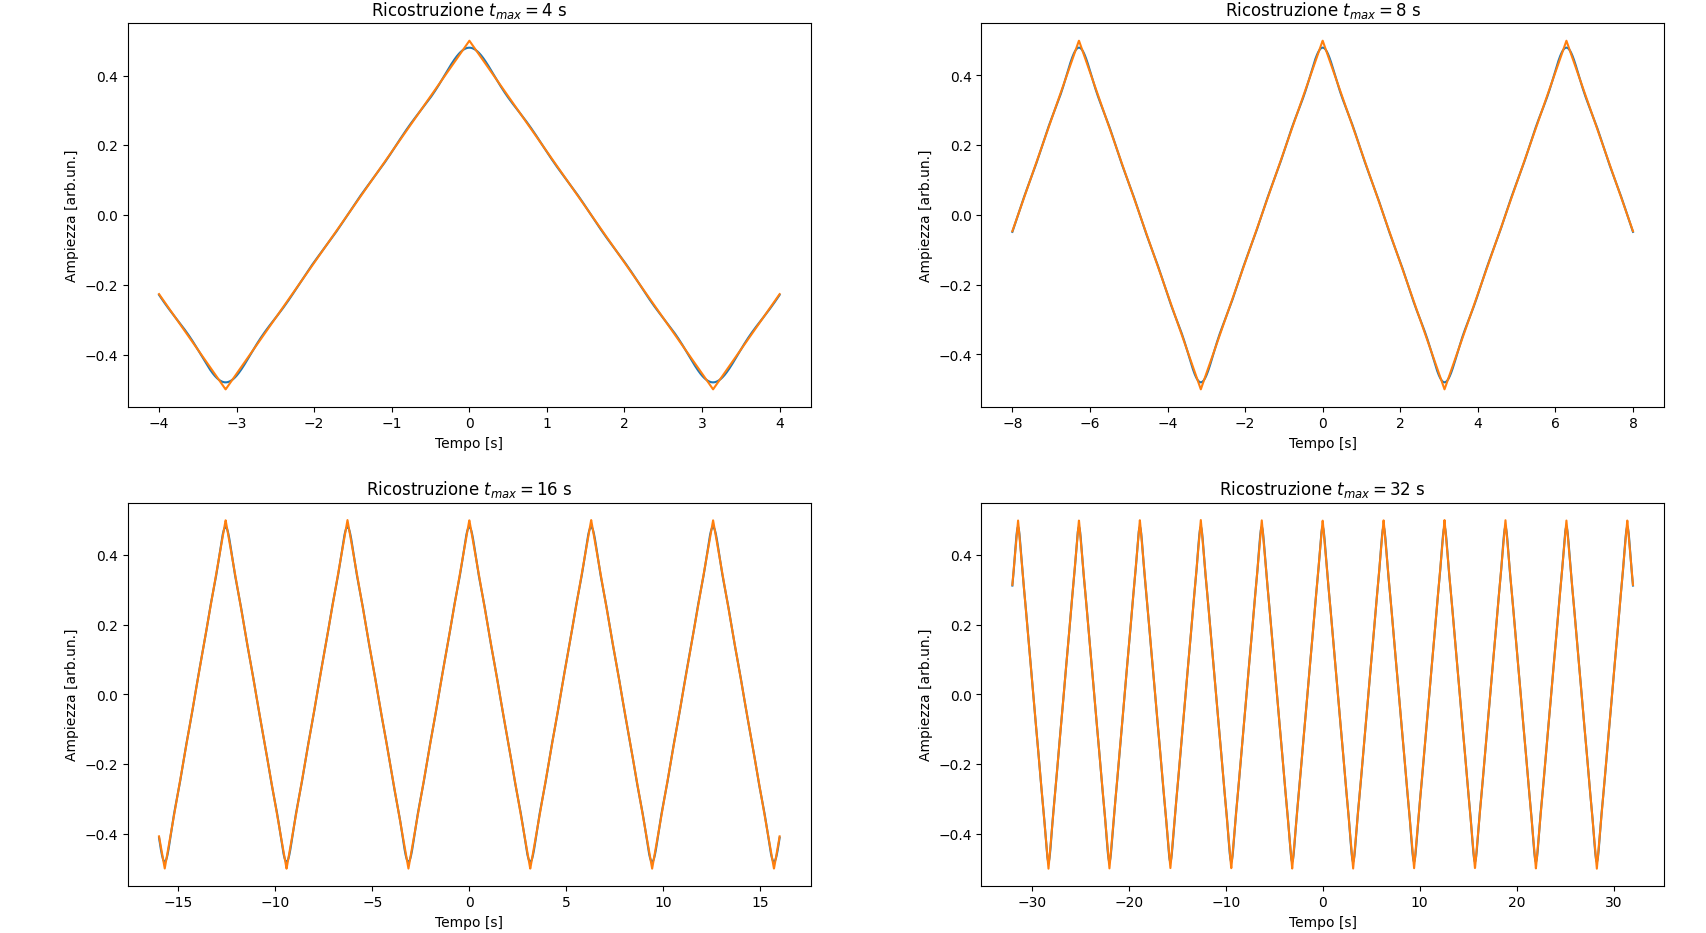
\includegraphics[width=0.84\textwidth]{img/Ricostruzione_onda_triangolare_campionamento.png}
            \caption{Ricostruzioni al variare di $t_{max}$, per $n=10$.}
            \label{Fig_OTC}
        \end{figure}

    \subsection{Analisi quantitativa}
    Per determinare quantitativamente la bontà delle ricostruzioni, abbiamo due possibili metodi. Il primo consiste nel calcolare la somma dei residui quadrati normalizzati (che indicheremo con $\chi^2_{\text{norm}}$), mentre il secondo nel calcolare l'integrale della differenza quadrata fra l'onda e la sua approssimazione (che indicheremo con $\Tilde{\chi}^2$). Il secondo metodo, che è la versione continua del primo, ha il vantaggio di avere precisione teoricamente infinita, mentre il primo avrebbe problemi con frequenze maggiori di quella di sampling. Tuttavia, questo secondo metodo è applicabile solo in questo caso di forme d'onda idealizzate. Quando più avanti lavoreremo con dati reali, che sono necessariamente discreti, dovremo per forza utilizzare il primo metodo. Qui riportiamo i risultati di entrambi i metodi per tutti i grafici eseguiti prima:
    \begin{itemize}
    
        \item Onda quadra:
            \begin{center}
    \begin{tabular}{|c|c|}
        \hline
        \multicolumn{2}{|c|}{Dati Fig. \ref{Fig_OQT}}\\
        \hline
        $\chi^2_{\text{norm}} = 0.01584$ & $\chi^2_{\text{norm}} = 1.912\cdot10^{-3}$ \\
        $\Tilde{\chi}^2 = 0.01584 $ & $\Tilde{\chi}^2 = 1.911\cdot10^{-3}$\\
        \hline
        $\chi^2_{\text{norm}} = 2.047\cdot10^{-4}$ & $\chi^2_{\text{norm}} = 7.964\cdot10^{-5}$ \\
        $\Tilde{\chi}^2 = 2.046\cdot10^{-4}$ & $\Tilde{\chi}^2 =7.964\cdot10^{-5}$\\
        \hline
    \end{tabular}
    
    \begin{tabular}{|c|c|}
        \hline
        \multicolumn{2}{|c|}{Dati Fig. \ref{Fig_OQC}}\\
        \hline
        $\chi^2_{\text{norm}} = 1.190\cdot10^{-3}$ & $\chi^2_{\text{norm}} = 9.947\cdot10^{-4}$\\
        $\Tilde{\chi}^2 = 1.193\cdot10^{-3}$ & $\Tilde{\chi}^2 = 9.948\cdot10^{-4}$\\
        \hline
        $\chi^2_{\text{norm}} = 1.086\cdot10^{-3}$ & $\chi^2_{\text{norm}} = 1.046\cdot10^{-3}$\\
        $\Tilde{\chi}^2 = 1.093\cdot10^{-3}$ & $\Tilde{\chi}^2 = 1.044\cdot10^{-3}$\\
        \hline
    \end{tabular}
            \end{center}

            
        \item Onda triangolare:
            \begin{center}
    \begin{tabular}{|c|c|}
        \hline
        \multicolumn{2}{|c|}{Dati Fig. \ref{Fig_OTT}}\\
        \hline
        $\chi^2_{\text{norm}} = 6.811\cdot10^{-5}$ & $\chi^2_{\text{norm}} = 1.280\cdot10^{-7}$ \\
        $\Tilde{\chi}^2 = 6.812\cdot10^{-5}$ & $\Tilde{\chi}^2 = 1.282\cdot10^{-7}$\\
        \hline
        $\chi^2_{\text{norm}} = 1.110\cdot10^{-10}$ & $\chi^2_{\text{norm}} = 4.926\cdot10^{-14}$ \\
        $\Tilde{\chi}^2 = 1.112\cdot10^{-10}$ & $\Tilde{\chi}^2 = 4.927\cdot10^{-14}$\\
        \hline
    \end{tabular}
    \quad
    \begin{tabular}{|c|c|}
        \hline
        \multicolumn{2}{|c|}{Dati Fig. \ref{Fig_OTTB}}\\
        \hline
        $\chi^2_{\text{norm}} = 0.001284$ & $\chi^2_{\text{norm}} = 2.136\cdot{10^-3}$\\
        $\Tilde{\chi}^2 = 0.001284$ & $\Tilde{\chi}^2 = 2.136\cdot{10^-3}$\\
        \hline
        $\chi^2_{\text{norm}} = 6.811\cdot10^{-5}$ & $\chi^2_{\text{norm}} = 1.543\cdot10^{-5}$\\
        $\Tilde{\chi}^2 = 6.812\cdot10^{-5}$ & $\Tilde{\chi}^2 = 1.544\cdot10^{-5}$\\
        \hline
    \end{tabular}
    \quad
    \begin{tabular}{|c|c|}
        \hline
        \multicolumn{2}{|c|}{Dati Fig. \ref{Fig_OTC}}\\
        \hline
        $\chi^2_{\text{norm}} = 1.543\cdot10^{-5}$ & $\chi^2_{\text{norm}} = 1.321\cdot10^{-5}$\\
        $\Tilde{\chi}^2 = 1.544\cdot10^{-5}$ & $\Tilde{\chi}^2 = 1.321\cdot10^{-5}$\\
        \hline
        $\chi^2_{\text{norm}} = 1.419\cdot10^{-5}$ & $\chi^2_{\text{norm}} = 1.376\cdot10^{-5}$\\
        $\Tilde{\chi}^2 = 1.419\cdot10^{-5}$ & $\Tilde{\chi}^2 = 1.376\cdot10^{-5}$\\
        \hline
    \end{tabular}
            \end{center}
    \end{itemize}
        
\section{Ricostruzione numerica pinna di squalo}
    Quando una forma d'onda quadra passa attraverso un integratore, le varie componenti armoniche vengono indipendentemente sfasate e riscalate, con guadagno e sfasamento dati da:
    \begin{align*}
        G(f) &= \frac{1}{\sqrt{1+(f/f_T)^2}}\\
        \Delta\phi(f) &= \arctan(-f/f_T)
    \end{align*}
    Per cui l'onda in uscita avrà espansione in serie di Fourier data da:
    \begin{equation}\label{eq-pinna}
        w(t) = \sum_{{k=1}\atop{k \text{ dispari}}}^n \frac{2}{k\pi} G(f_k) \sin\left(2\pi f_k t + \Delta\phi(f_k)\right)
    \end{equation}
    dove le $f_k = kf$ sono le armoniche della frequenza $f$ dell'onda originaria.\\ Abbiamo ricostruito numericamente gli andamenti in uscita a varie frequenze, lasciando la frequenza di taglio $f_T = 482$ Hz (scelta poiché uguale al valore nominale di $f_T$ usato nella sezione successiva).\\
    Possiamo notare dai grafici che, come ci si attende, per $f<f_T$ l'onda rimane quasi indisturbata, mentre al crescere di $f$ l'onda diminuisce di ampiezza e si deforma, arrivando ad assomigliare ad un'onda triangolare. Notiamo inoltre come la forma d'onda triangolare per $f\gg f_T$ risulta essere sfasata di un quarto di periodo.
    \begin{figure}[H]
        \centering
        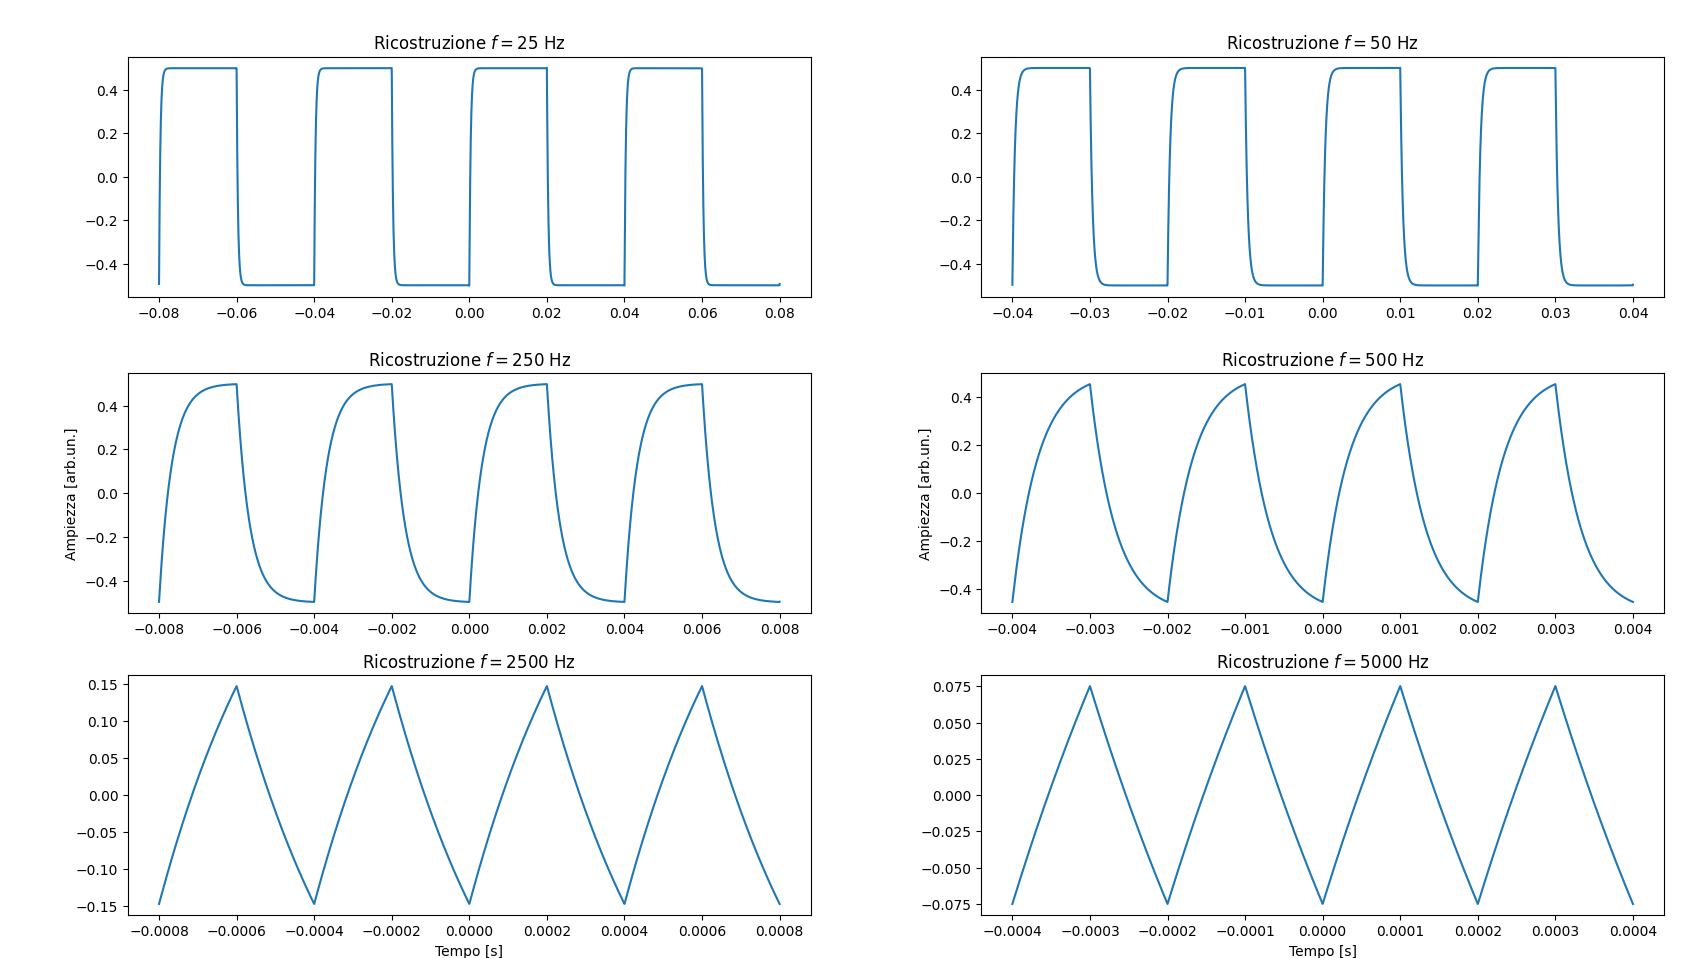
\includegraphics[width=0.9\textwidth]{img/Ricostruzione_pinna.png}
        \caption{Ricostruzioni al variare di $f$, per $f_T = 482$ Hz.}
    \end{figure}

\section{Best-fit pinna di squalo}
    \noindent A lezione abbiamo misurato con Arduino la d.d.p. in uscita da un integratore in funzione del tempo per tre onde quadre di diversa frequenza in entrata. La resistenza nominale usata per l'integratore vale $R=0.33$ k$\Omega$ ($\pm 10\%$) e la capacità nominale del condensatore $C=1$ $\mu$F ($\pm 10\%$), da cui otteniamo un valore nominale per la frequenza di taglio di $f_T=482$ Hz.\\
    Abbiamo eseguito un best fit del minimo $\chi^2$ per una forma d'onda del tipo (\ref{eq-pinna}) sui dati ottenuti tramite Arduino. Abbiamo usato come parametri di fit: la frequenza $f$, l'ampiezza $A$ dell'onda originaria, l'offset $C$ e lo sfasamento $\phi_0$. Riportiamo i grafici e i risultati per le tre prese dati:
    
    \begin{figure}[H]
        \centering
        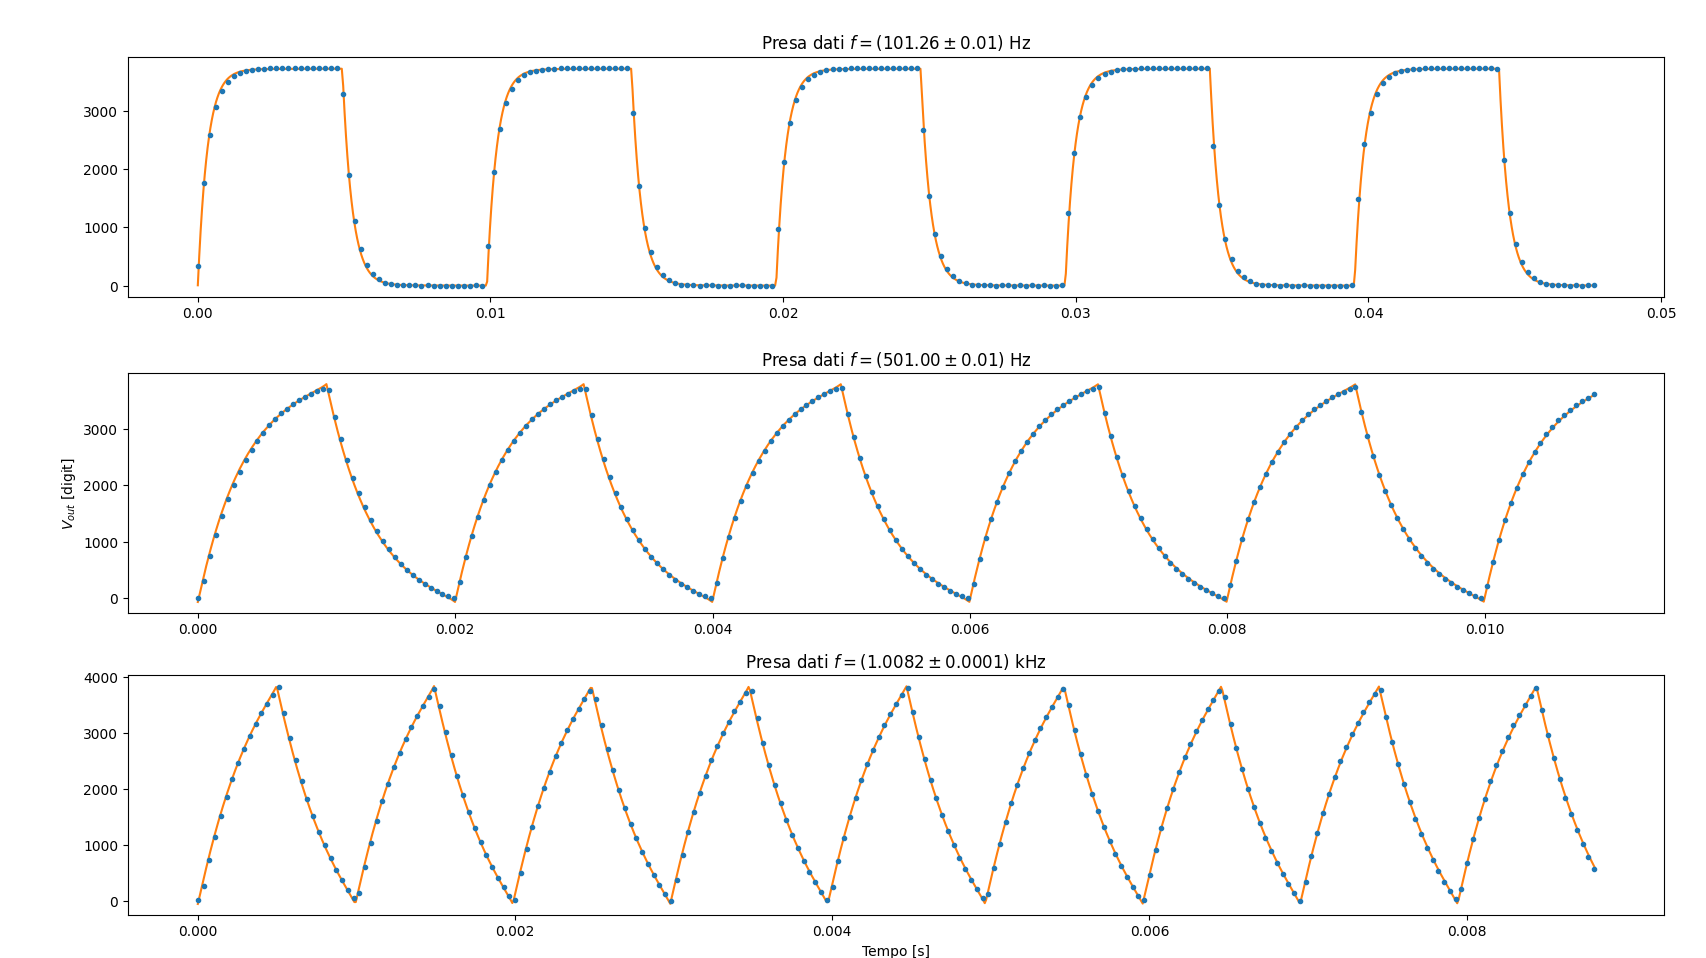
\includegraphics[width=0.9\textwidth]{img/Fit.png}
        \caption{Grafici dei fit}
    \end{figure}
    \begin{itemize}
        \item Presa dati $f=(101.26\pm0.01)$ Hz:
        \begin{align*}
            w(t) &= C + \sum_{{k=1}\atop{k \text{ dispari}}}^n \frac{2A}{k\pi} G(f_k) \sin\left(2\pi f_k t + \Delta\phi(f_k) + \phi_0\right)\\
            f &=  (101.2076 \pm 0.0002) \text{ Hz}\\
            A &=  (3723.09 \pm 0.05) \text{ digit} \\
            C &=  (1861.77 \pm 0.03) \text{ digit}\\
            \phi_0 &=  -(0.000651 \pm 0.000006) \text{ rad} \\
            \kappa^2 &=  488039 \\
            ndof &=  232 \\
            \kappa^2_{norm} &= 2104 \\
            \texttt{absolute\_sigma} &= \texttt{True}
        \end{align*}
            
        \item Presa dati $f=(501.00\pm0.01)$ Hz:
        \begin{align*}
            w(t) &= C + \sum_{{k=1}\atop{k \text{ dispari}}}^n \frac{2A}{k\pi} G(f_k) \sin\left(2\pi f_k t + \Delta\phi(f_k) + \phi_0\right)\\
            f &=  (500.349 \pm 0.003) \text{ Hz} \\
            A &=  (4003.4 \pm 0.2)\text{ digit} \\
            C &=  (1858.26 \pm 0.06) \text{ digit} \\
            \phi_0 &=  -(0.0908 \pm 0.0001) \text{ rad} \\
            \kappa^2 &=  82621\\
            ndof &=  235 \\
            \kappa^2_{norm} &= 351.58\\
            \texttt{absolute\_sigma} &= \texttt{True}
        \end{align*}
        
        \item Presa dati $f=(1.0082\pm0.0001)$ kHz:
        \begin{align*}
            w(t) &= C + \sum_{{k=1}\atop{k \text{ dispari}}}^n \frac{2A}{k\pi} G(f_k) \sin\left(2\pi f_k t + \Delta\phi(f_k) + \phi_0\right)\\
            f &=  (1.00724 \pm 0.00001) \text{ kHz}\\
            A &=  (5901 \pm 1) \text{ digit} \\
            C &=  (1894.4 \pm 0.2) \text{ digit} \\
            \phi_0 &=  -(0.1047 \pm 0.0004) \text{ rad} \\
            \kappa^2 &=  13483 \\
            ndof &=  243 \\
            \kappa^2_{norm} &= 55.48\\
            \texttt{absolute\_sigma} &= \texttt{True}
        \end{align*}
    \end{itemize}
    
\section{Simulazione numerica dei grafici guadagno \textit{VS} frequenza}

    Abbiamo ricostruito il guadagno per l'integratore con forma d'onda quadra in ingresso, simulando numericamente il segnale in uscita come sopra da (\ref{eq-pinna}) e calcolandone l'ampiezza picco-picco. Come sopra abbiamo usato come valore per la frequenza di taglio pari a $f_T=482$ Hz.\\
   
    \begin{figure}[H]
        \centering
        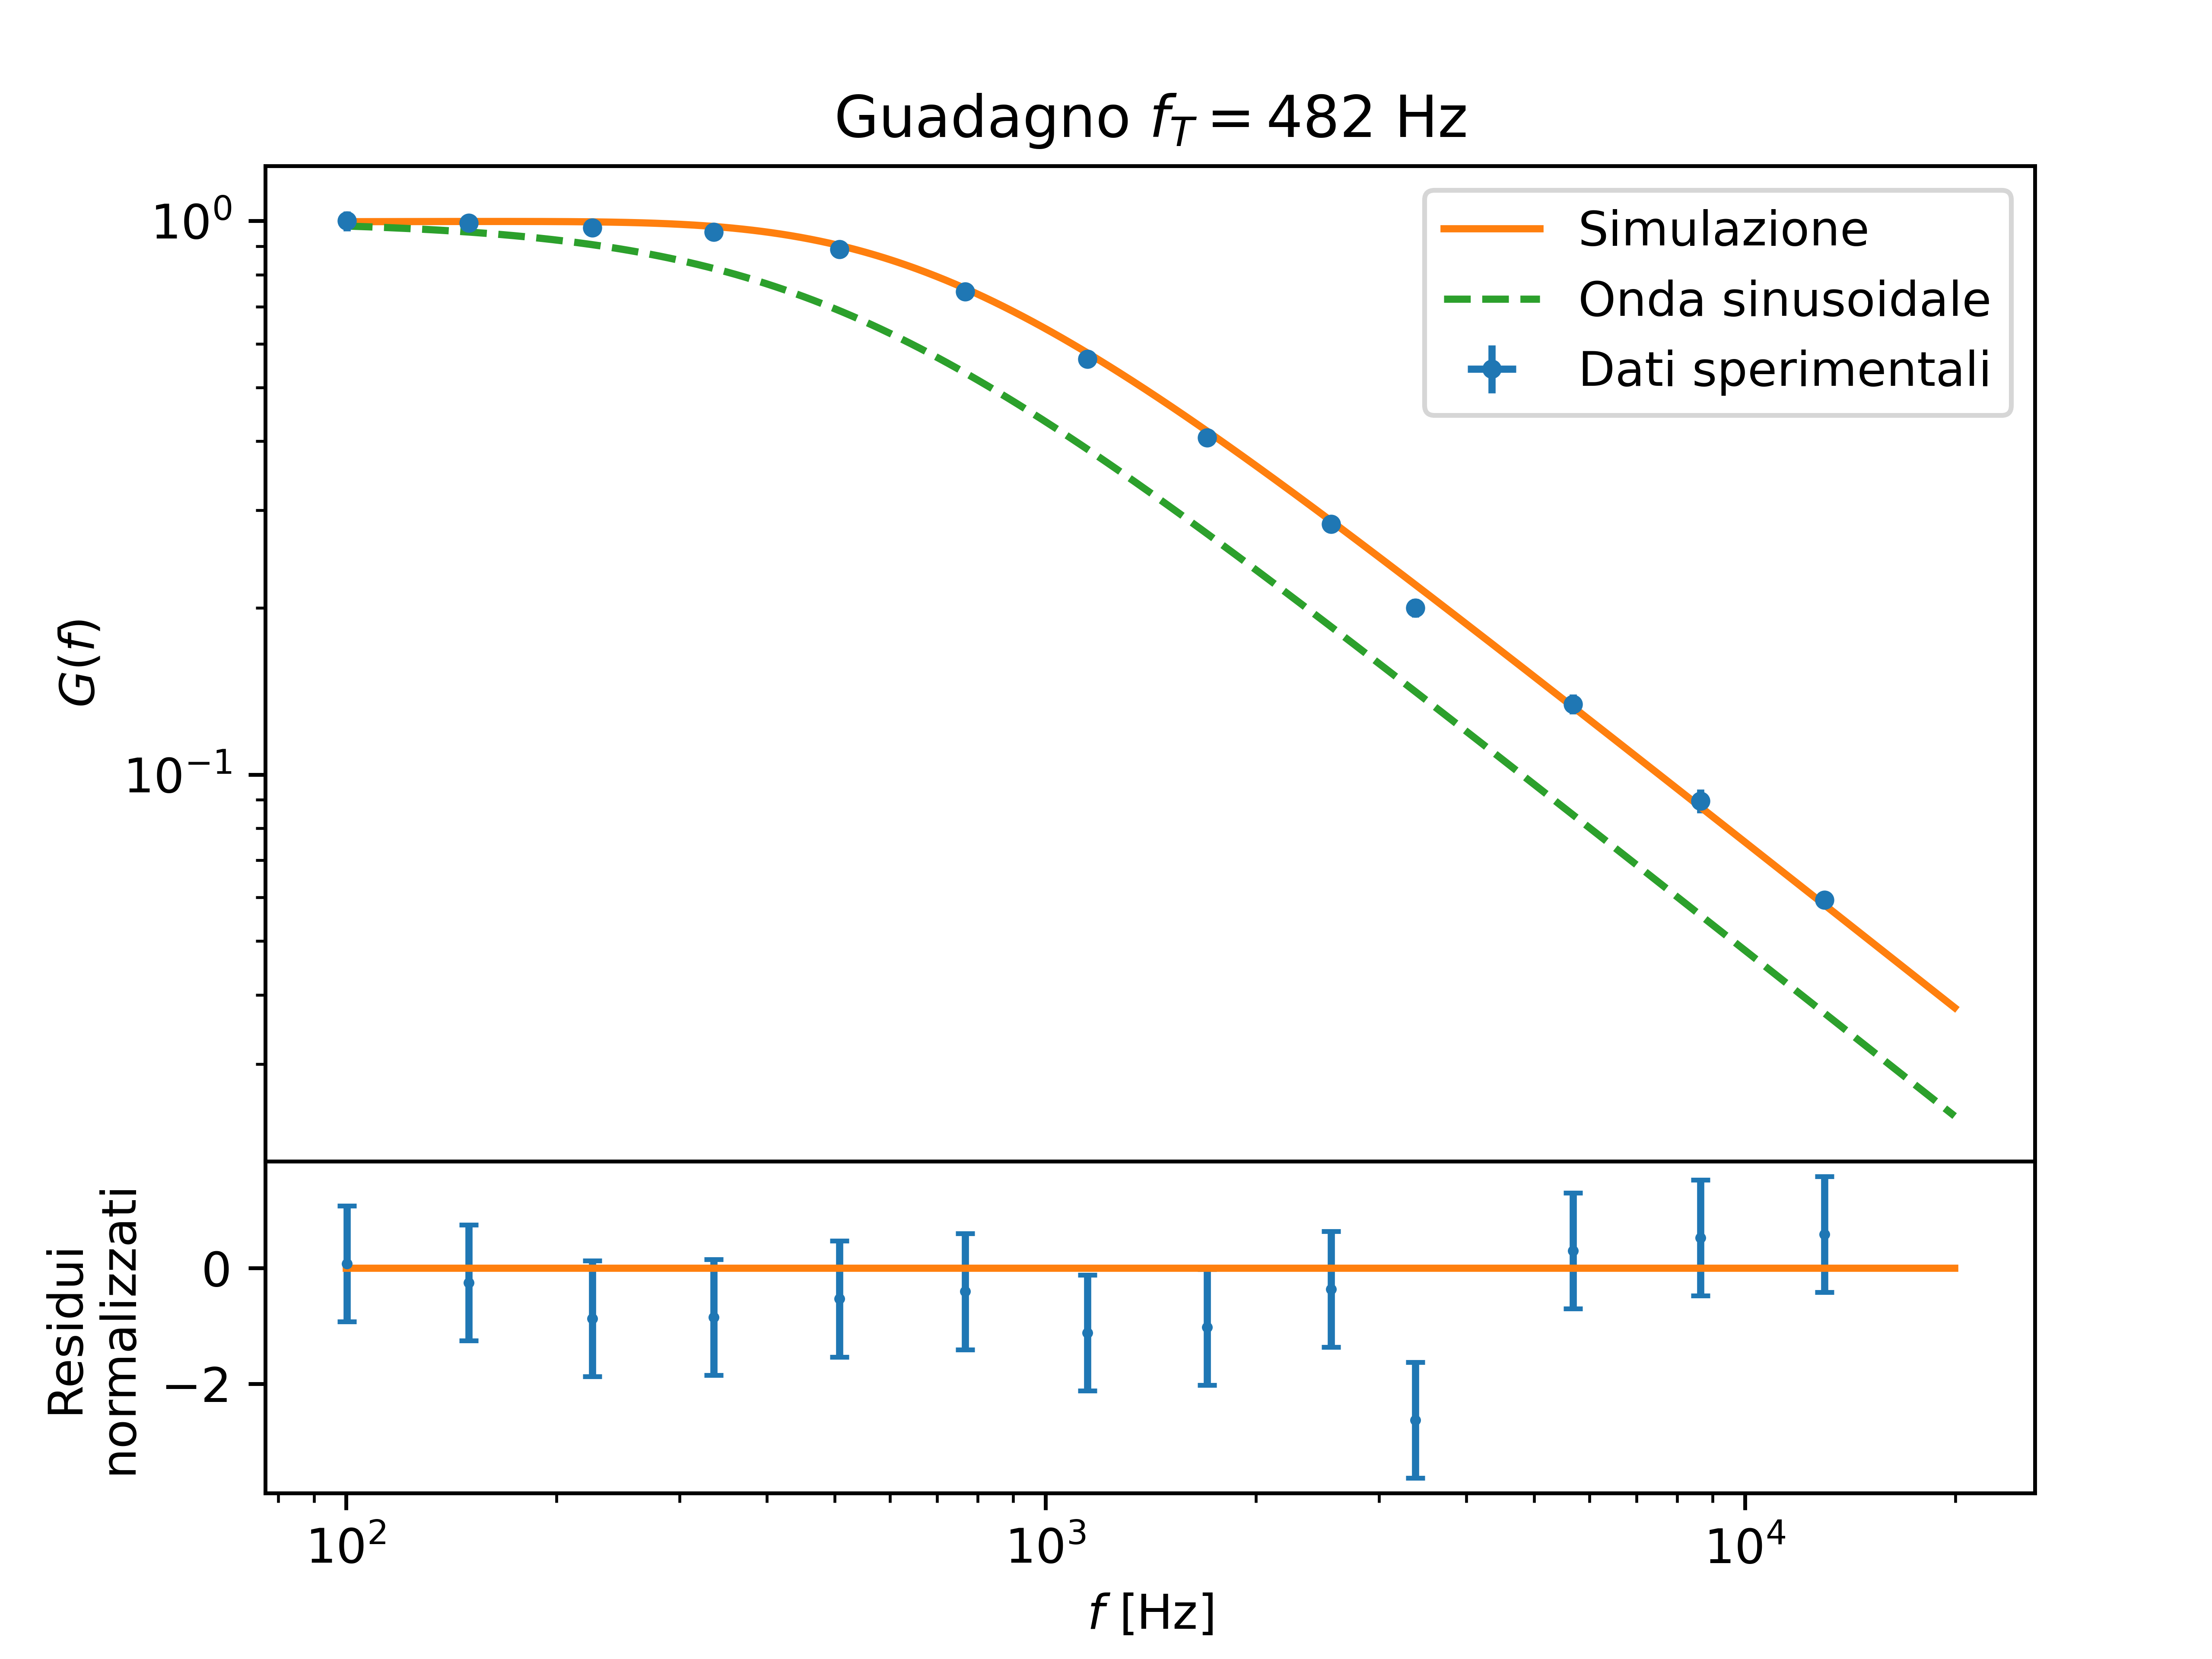
\includegraphics[width=0.9\textwidth]{img/Guadagno.png}
        \caption{Grafico guadagno $G(f)$ per $f_T=482$ Hz.}
    \end{figure}
    
    \noindent Dal grafico si nota come l'andamento sperimentale è ben approssimato dalla simulazione, mentre si discosta significativamente da quello atteso per un'onda sinusoidale. In realtà ci aspetteremmo una piccola perturbazione dovuta alla resistenza interna dell'oscilloscopio, che evidentemente si è rivelata trascurabile. Possiamo quantificare l'effetto di tale resistenza per verificare teoricamente questo fatto.\\
    Chiamando $R_{osc}$ la resistenza interna dell'oscilloscopio, la correzione al primo ordine all'espressione del guadagno dovuta al contributo dell'oscilloscopio per una frequenza $f$ è data da:
    \[|\Delta G(f)|= \left(\frac{1}{1+f^2/f_T^2}\right)^{\frac{3}{2}} \frac{1}{2\pi f_TR_{osc}C}\]
    Riportiamo in appendice alla relazione la derivazione di questa espressione.\\
    Affinché l'effetto della resistenza interna dell'oscilloscopio sia trascurabile, la correzione al guadagno per le onde quadre deve essere minore dell'errore sulla misura del guadagno. Di seguito riportiamo un grafico in cui confrontiamo $\Delta G$ per le fondamentali delle onde misurate con gli errori sulle corrispettive misure dei guadagni.

    \begin{figure}[H]
        \centering
        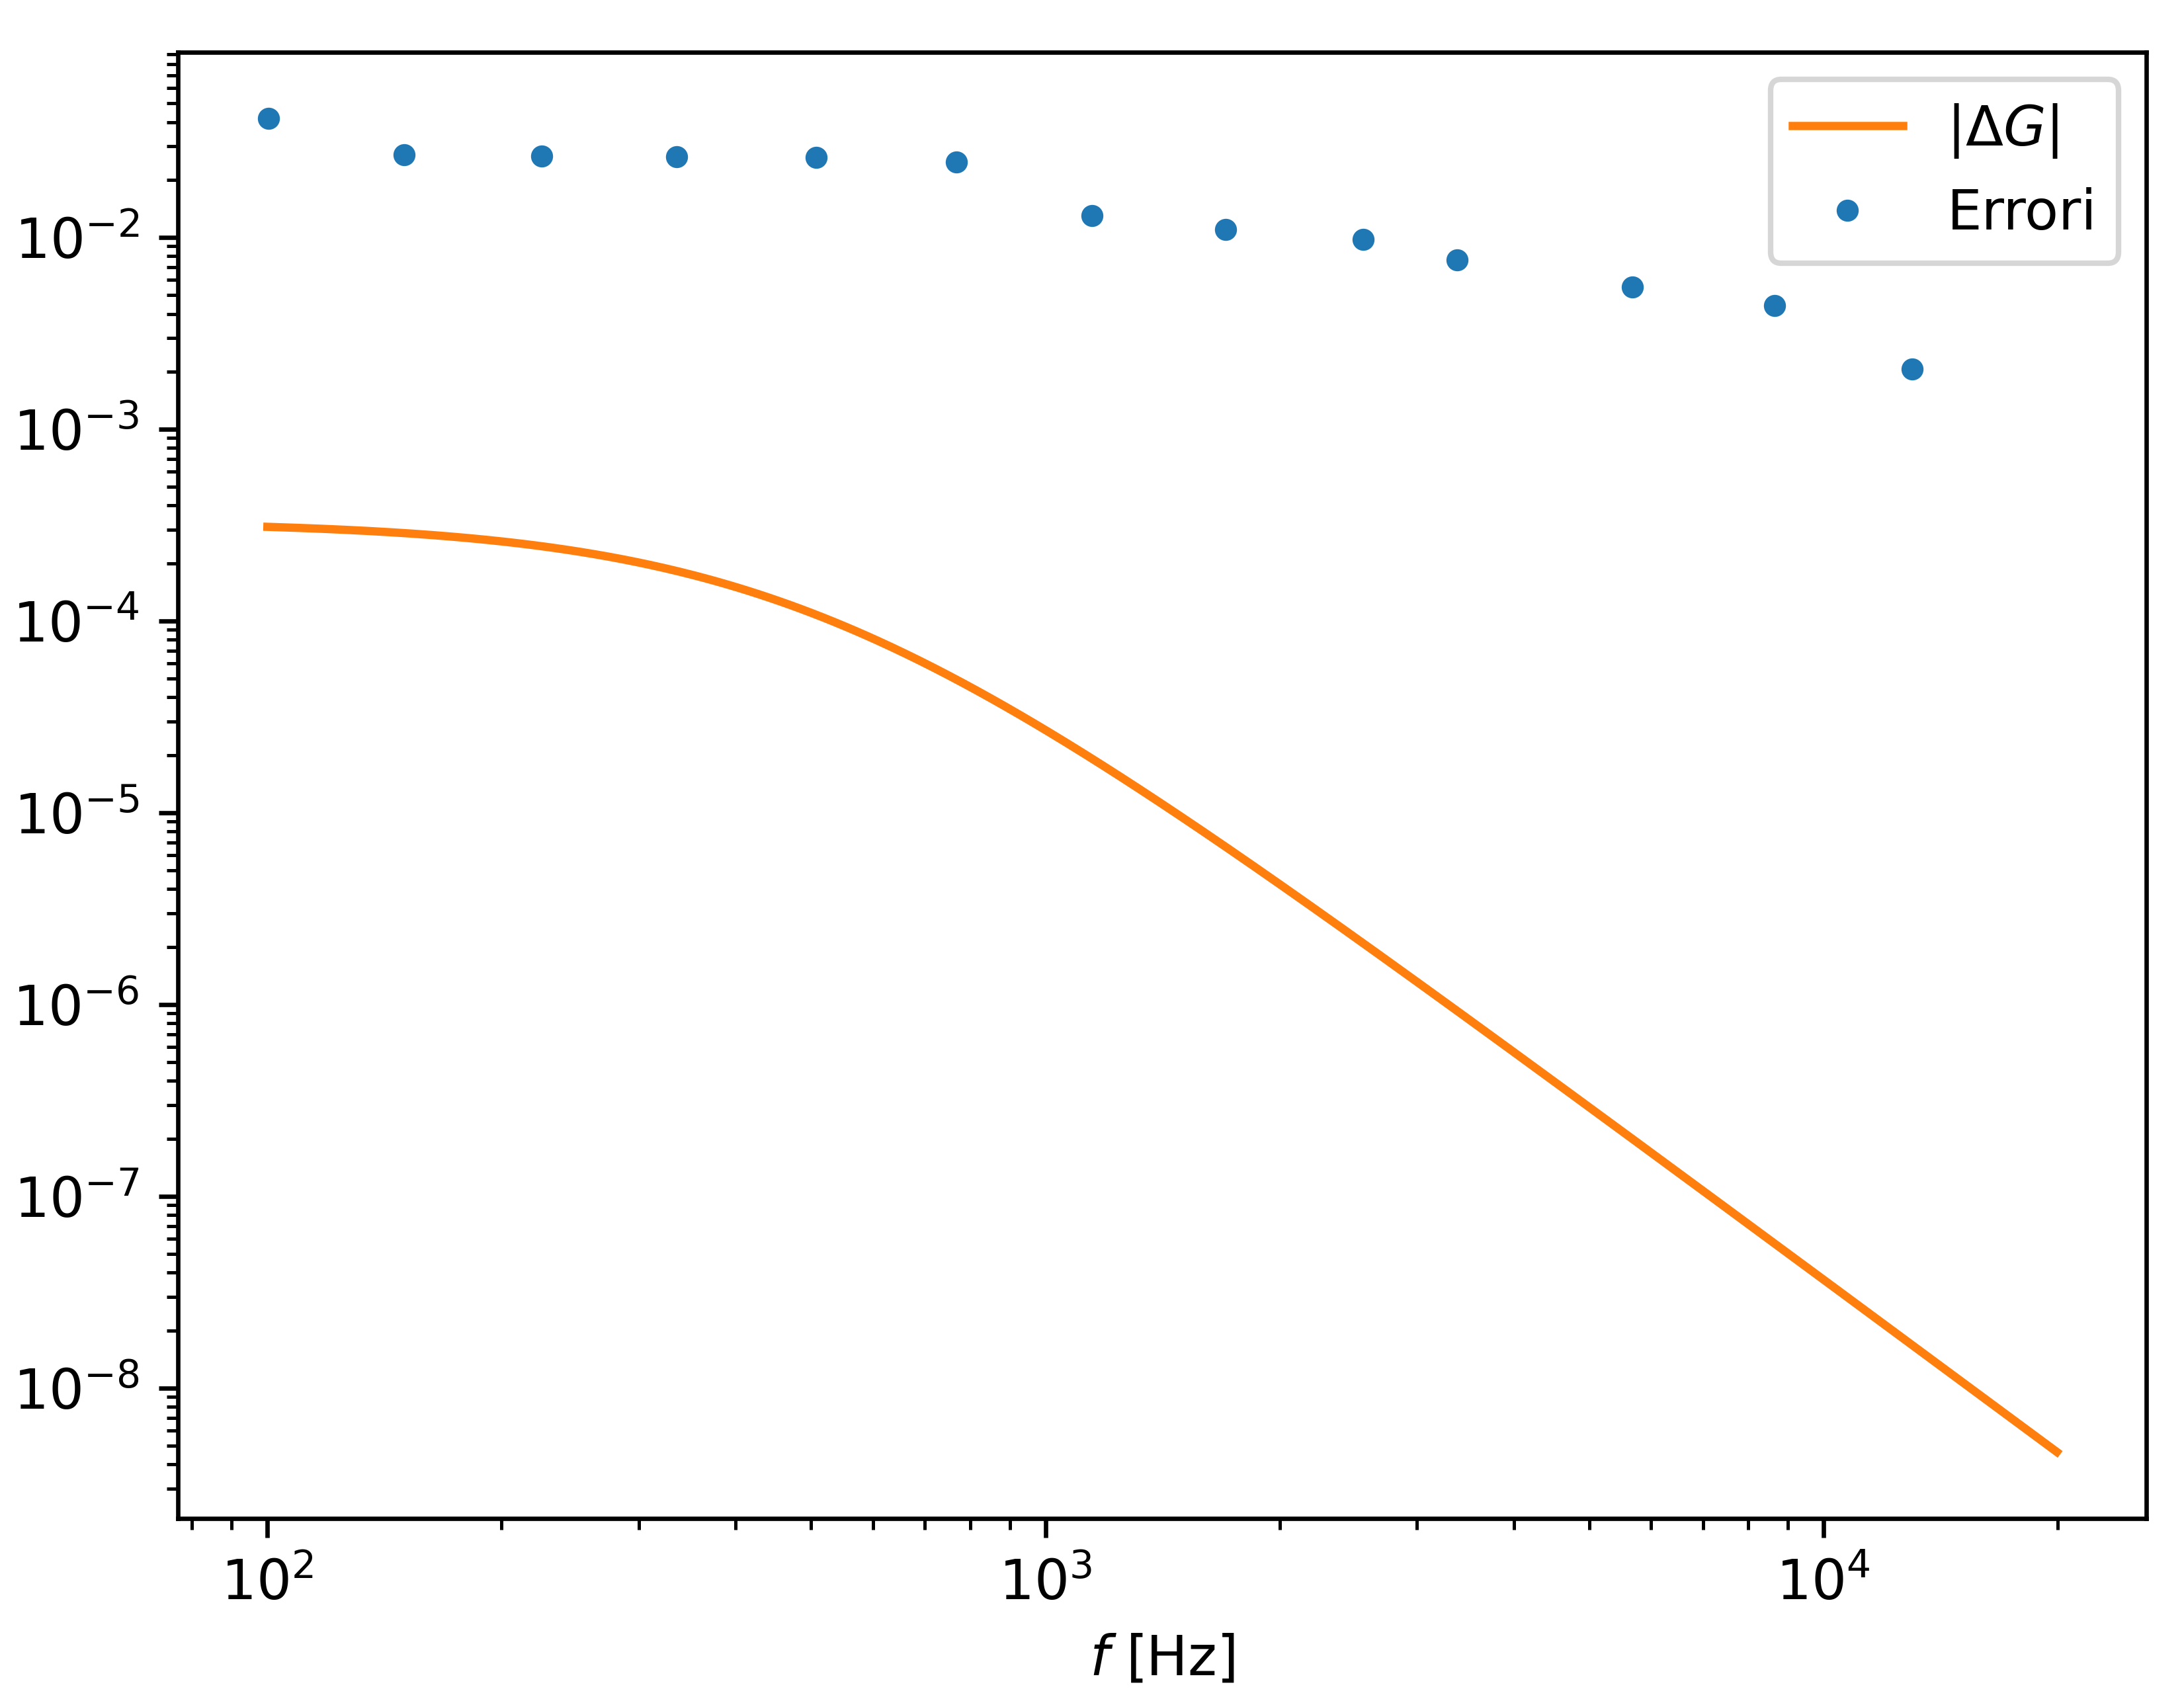
\includegraphics[width=0.90\textwidth]{img/correzione.png}
        \caption{Confronto tra $|\Delta G|$ e errore sul guadagno per le varie misure.}
    \end{figure}
    
    \noindent Come risulta evidente dal grafico, $\Delta G$ per la fondamentale risulta trascurabile rispetto agli errori per tutte le misure. Poiché $\Delta G$ per le armoniche successive risulta molto minore rispetto alla fondamentale, troviamo che era effettivamente atteso che la resistenza del generatore risulti trascurabile.
    
\section{Idem con onda triangolare in ingresso}

    \subsection{Ricostruzione onda in uscita da integratore}
        Analogamente all'onda quadra, quando un'onda triangolare passa attraverso un integratore, l'onda in uscita avrà espansione in serie di Fourier data da:
        \begin{equation}\label{eq-pinna-T}
        w(t) = \sum_{{k=1}\atop{k \text{ dispari}}}^n \left(\frac{2}{k\pi}\right)^2 G(f_k) \cos\left(2\pi f_k t + \Delta\phi(f_k)\right)
        \end{equation}
        Dove $G(f)$ e $\phi(f)$ sono come sopra, essendo caratteristiche del circuito.\\
        Come prima, abbiamo ricostruito numericamente gli andamenti in uscita a varie frequenze, sempre con frequenza di taglio $f_T = 482$ Hz.\\
        Come prima, possiamo notare dai grafici che per $f<f_T$ l'onda rimane quasi indisturbata, mentre al crescere di $f$ l'onda diminuisce di ampiezza e si deforma. In particolare stavolta, per $f\gg f_T$ le creste e le valli diventano archi parabolici e l'onda risulta essere sfasata di un quarto di periodo.
    
    \begin{figure}[H]
        \centering
        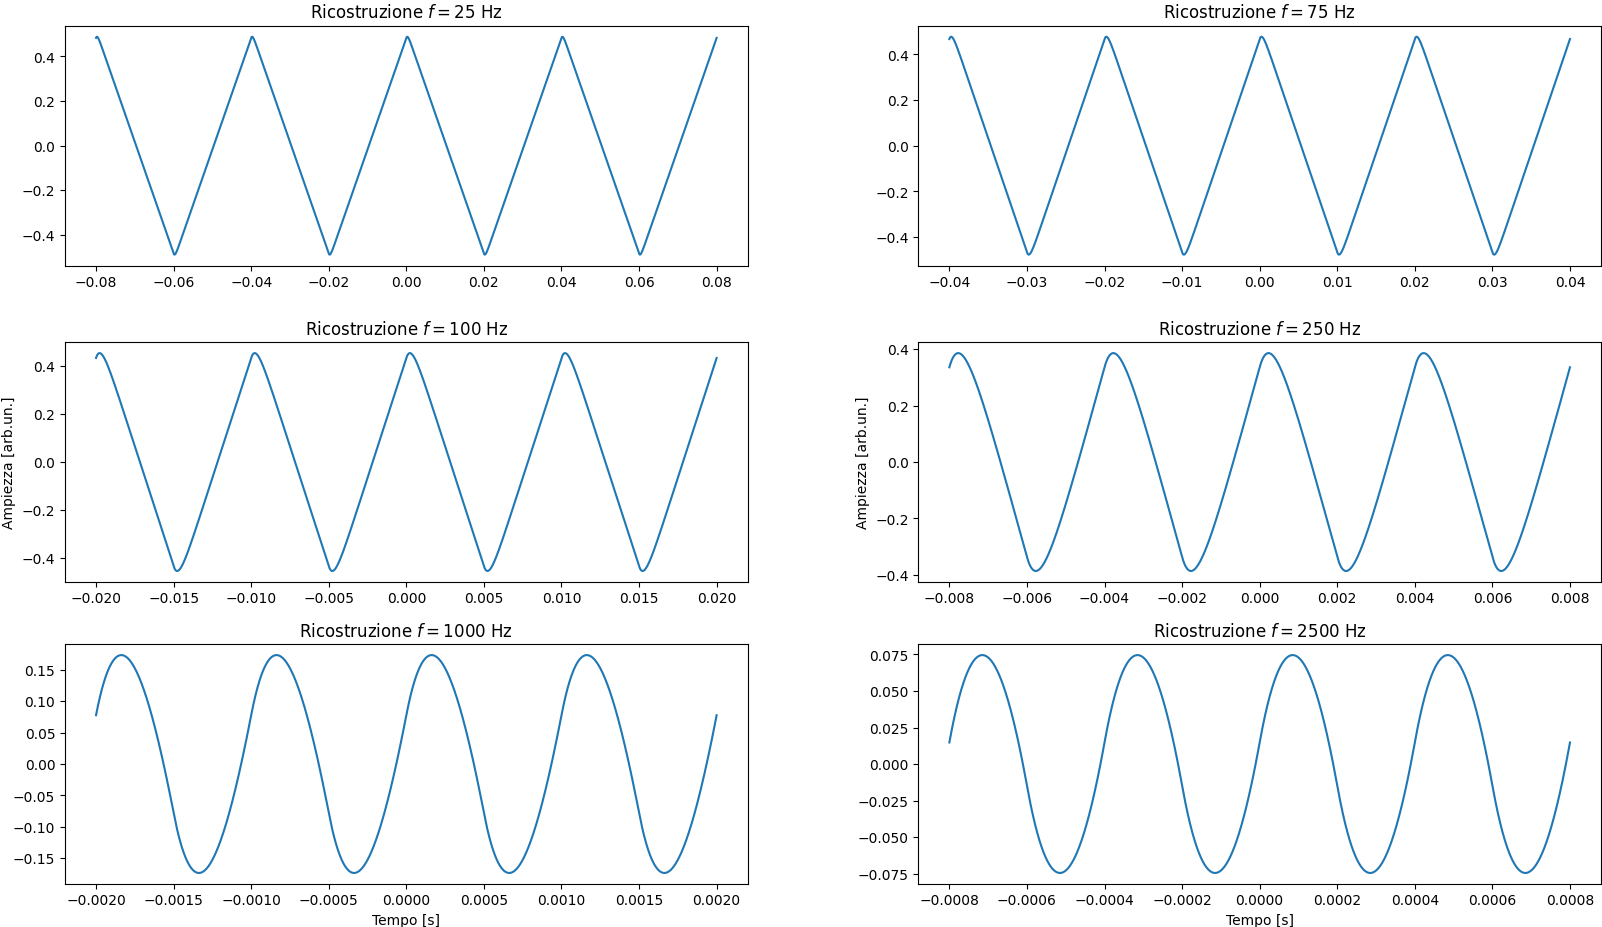
\includegraphics[width=0.9\textwidth]{img/Ricostruzione_pinna-T.png}
        \caption{Ricostruzioni al variare di $f$, per $f_T = 482$ Hz.}
    \end{figure}
    
    \subsection{Best-fit onda in uscita da integratore}
        Come fatto al punto 3, abbiamo eseguito un best fit del minimo $\chi^2$ per una forma d'onda del tipo (\ref{eq-pinna-T}) su due set di dati, ottenuti facendo passare onde triangolari attraverso lo stesso circuito descritto in precedenza. Riportiamo i grafici e i risultati per le due prese dati.
    
    \begin{figure}[H]
        \centering
        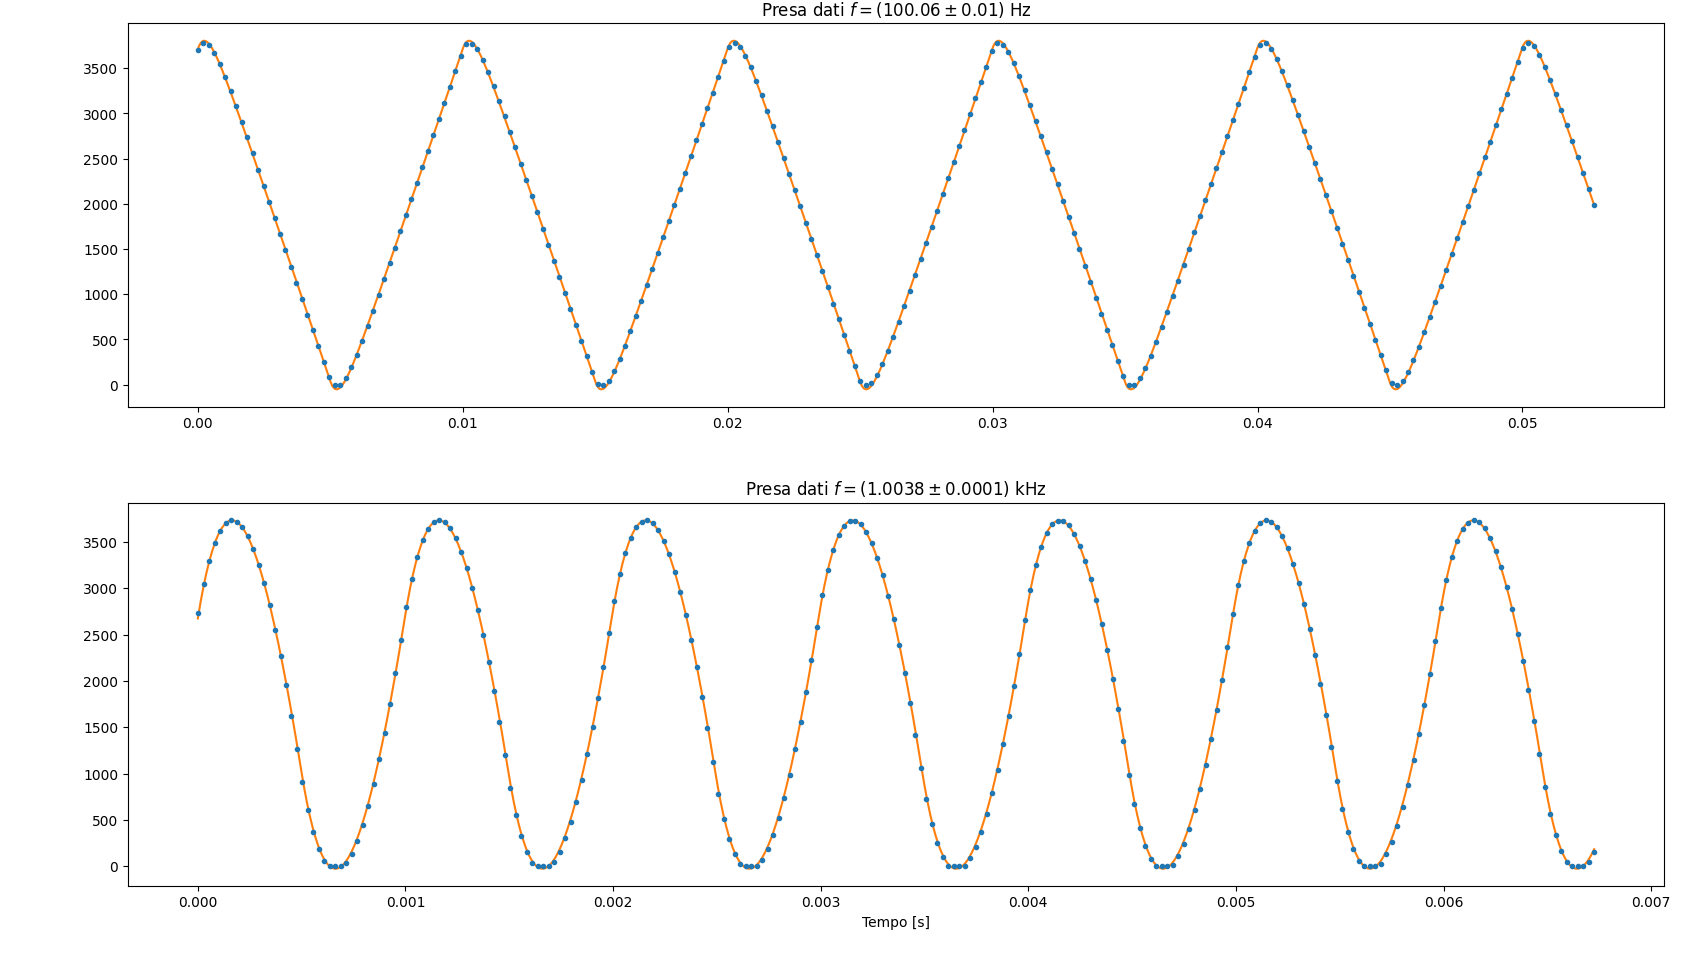
\includegraphics[width=0.9\textwidth]{img/Fit-T.png}
        \caption{Grafici dei fit.}
    \end{figure}

        \begin{itemize}
        \item Presa dati $f=(100.06\pm0.01)$ Hz:
        \begin{align*}
            w(t) &= \sum_{{k=1}\atop{k \text{ dispari}}}^n \left(\frac{2}{k\pi}\right)^2 G(f_k) \cos\left(2\pi f_k t + \Delta\phi(f_k)\right)\\
            f &=  (100.0637 \pm 0.0005) \text{ Hz}\\
            A &=  (4199.8 \pm 0.1) \text{ digit} \\
            C &=  (1886.29 \pm 0.05) \text{ digit} \\
            \phi_0 &=  -(0.02073 \pm 0.00009) \text{ rad} \\
            \kappa^2 &=  158622 \\
            ndof &=  256 \\
            \kappa^2_{norm} &= 620\\
            \texttt{absolute\_sigma} &= \texttt{True}
        \end{align*}
            
        \item Presa dati $f=(1.0038\pm0.0001)$ kHz:
        \begin{align*}
            w(t) &= \sum_{{k=1}\atop{k \text{ dispari}}}^n \left(\frac{2}{k\pi}\right)^2 G(f_k) \cos\left(2\pi f_k t + \Delta\phi(f_k)\right)\\
            f &=  (1.00363 \pm 0.00001) \text{ kHz} \\
            A &=  (10786.0 \pm 0.6)\text{ digit} \\
            C &=  (1858.83 \pm 0.09) \text{ digit} \\
            \phi_0 &=  -(0.0281 \pm 0.0003) \text{ rad} \\
            \kappa^2 &=  65175\\
            ndof &=  256 \\
            \kappa^2_{norm} &= 254.59\\
            \texttt{absolute\_sigma} &= \texttt{True}
        \end{align*}
    \end{itemize}

        \noindent Notiamo dai grafici che le valli delle forme d'onda risultano "appiattite". Controllando i valori acquisiti da Arduino, ci siamo resi conto che in quegli istanti era stata registrata una d.d.p. pari a 0. Arduino registra solo d.d.p. positive, ragione per cui avevamo introdotto manualmente un offset all'onda guardando il segnale sull'oscilloscopio durante la presa dati. Evidentemente, l'offset introdotto non era sufficiente e in quei tratti la d.d.p. era negativa, che è stata poi registrata come nulla da Arduino. Pertanto, abbiamo ripetuto i fit eliminando quei punti dal set. Riportiamo i grafici e i risultati del nuovo fit. 
        
    \begin{figure}[H]
        \centering
        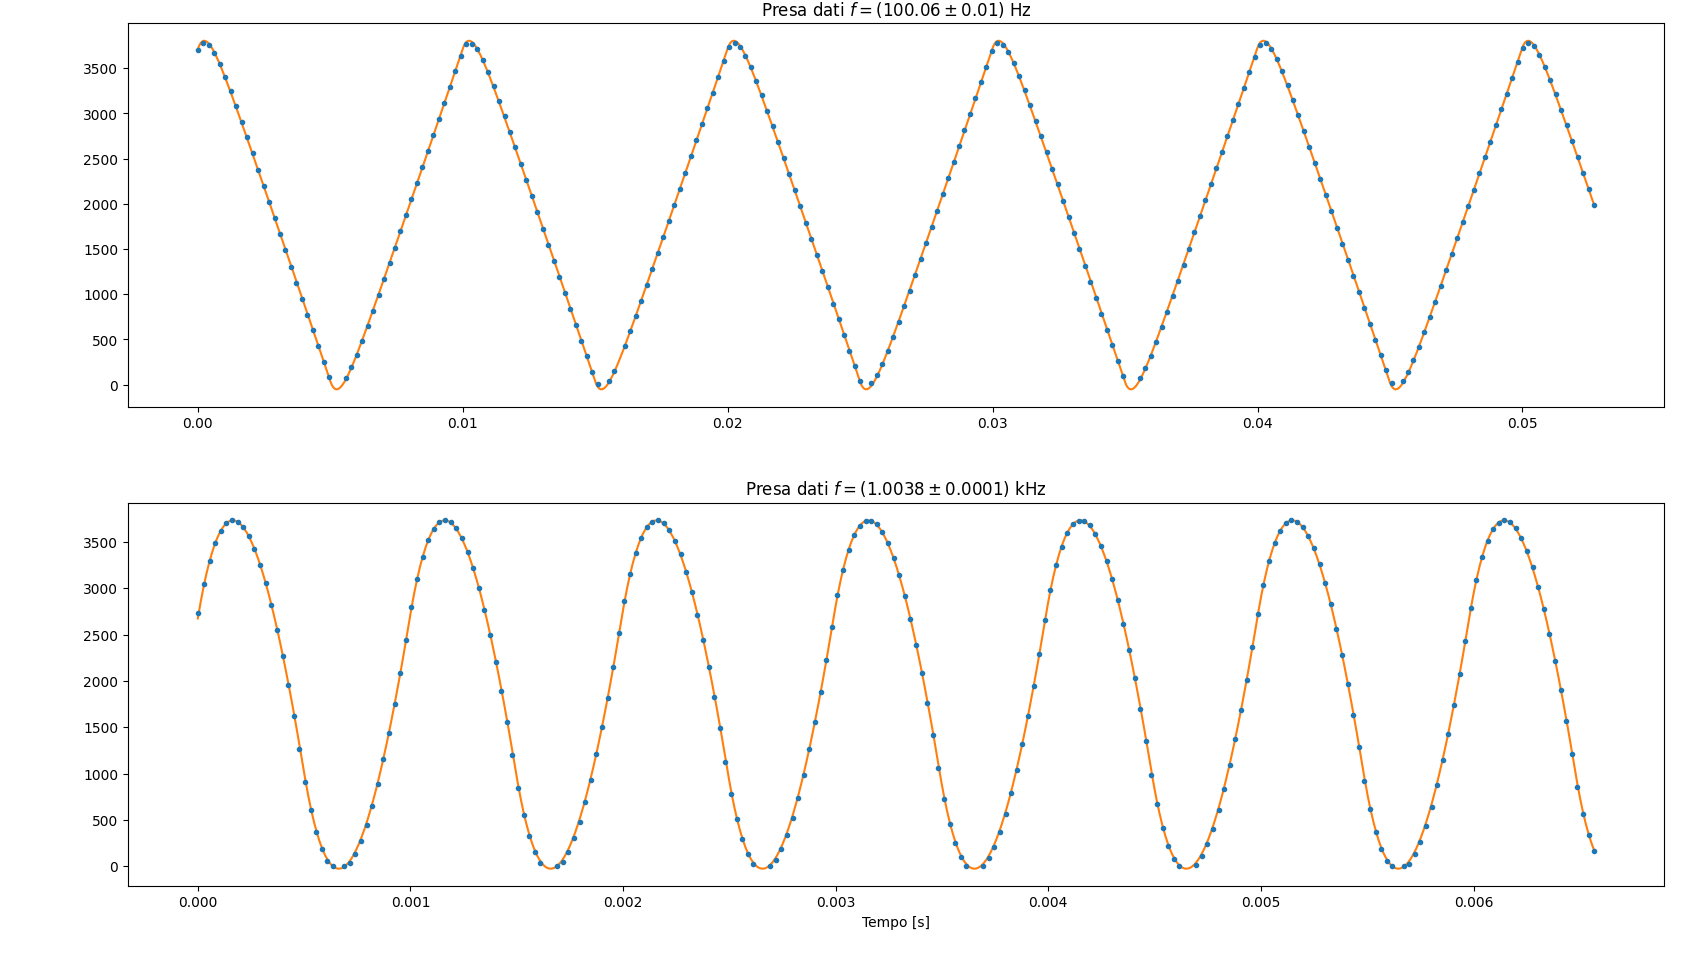
\includegraphics[width=0.9\textwidth]{img/Fit-T-tagliato.png}
        \caption{Grafici dei fit senza outliers.}
    \end{figure}

    \begin{itemize}
        \item Presa dati $f=(100.06\pm0.01)$ Hz:
        \begin{align*}
            w(t) &= \sum_{{k=1}\atop{k \text{ dispari}}}^n \left(\frac{2}{k\pi}\right)^2 G(f_k) \cos\left(2\pi f_k t + \Delta\phi(f_k)\right)\\
            f &=  (100.0573 \pm 0.0005) \text{ Hz}\\
            A &=  (4250.7 \pm 0.2) \text{ digit} \\
            C &=  (1876.11 \pm 0.06) \text{ digit} \\
            \phi_0 &=  -(0.01890 \pm 0.00009) \text{ rad} \\
            \kappa^2 &=  38959 \\
            ndof &=  248 \\
            \kappa^2_{norm} &= 157\\
            \texttt{absolute\_sigma} &= \texttt{True}
        \end{align*}
           
        \item Presa dati $f=(1.0038\pm0.0001)$ kHz:
        \begin{align*}
            w(t) &= \sum_{{k=1}\atop{k \text{ dispari}}}^n \left(\frac{2}{k\pi}\right)^2 G(f_k) \cos\left(2\pi f_k t + \Delta\phi(f_k)\right)\\
            f &=  (1.003457 \pm 0.000008) \text{ Hz} \\
            A &=  (10862.5 \pm 0.7)\text{ digit} \\
            C &=  (1852.87 \pm 0.09) \text{ digit} \\
            \phi_0 &=  -(0.0105 \pm 0.0003) \text{ rad} \\
            \kappa^2 &=  5397\\
            ndof &=  240 \\
            \kappa^2_{norm} &= 22.49\\
            \texttt{absolute\_sigma} &= \texttt{True}
        \end{align*}
    \end{itemize}
    \subsection{Simulazione numerica dei grafici guadagno \textit{VS} frequenza}
        Come al punto 4, abbiamo ricostruito il guadagno in uscita da un integratore, stavolta con un'onda triangolare in ingresso.
            \begin{figure}[H]
                \centering
                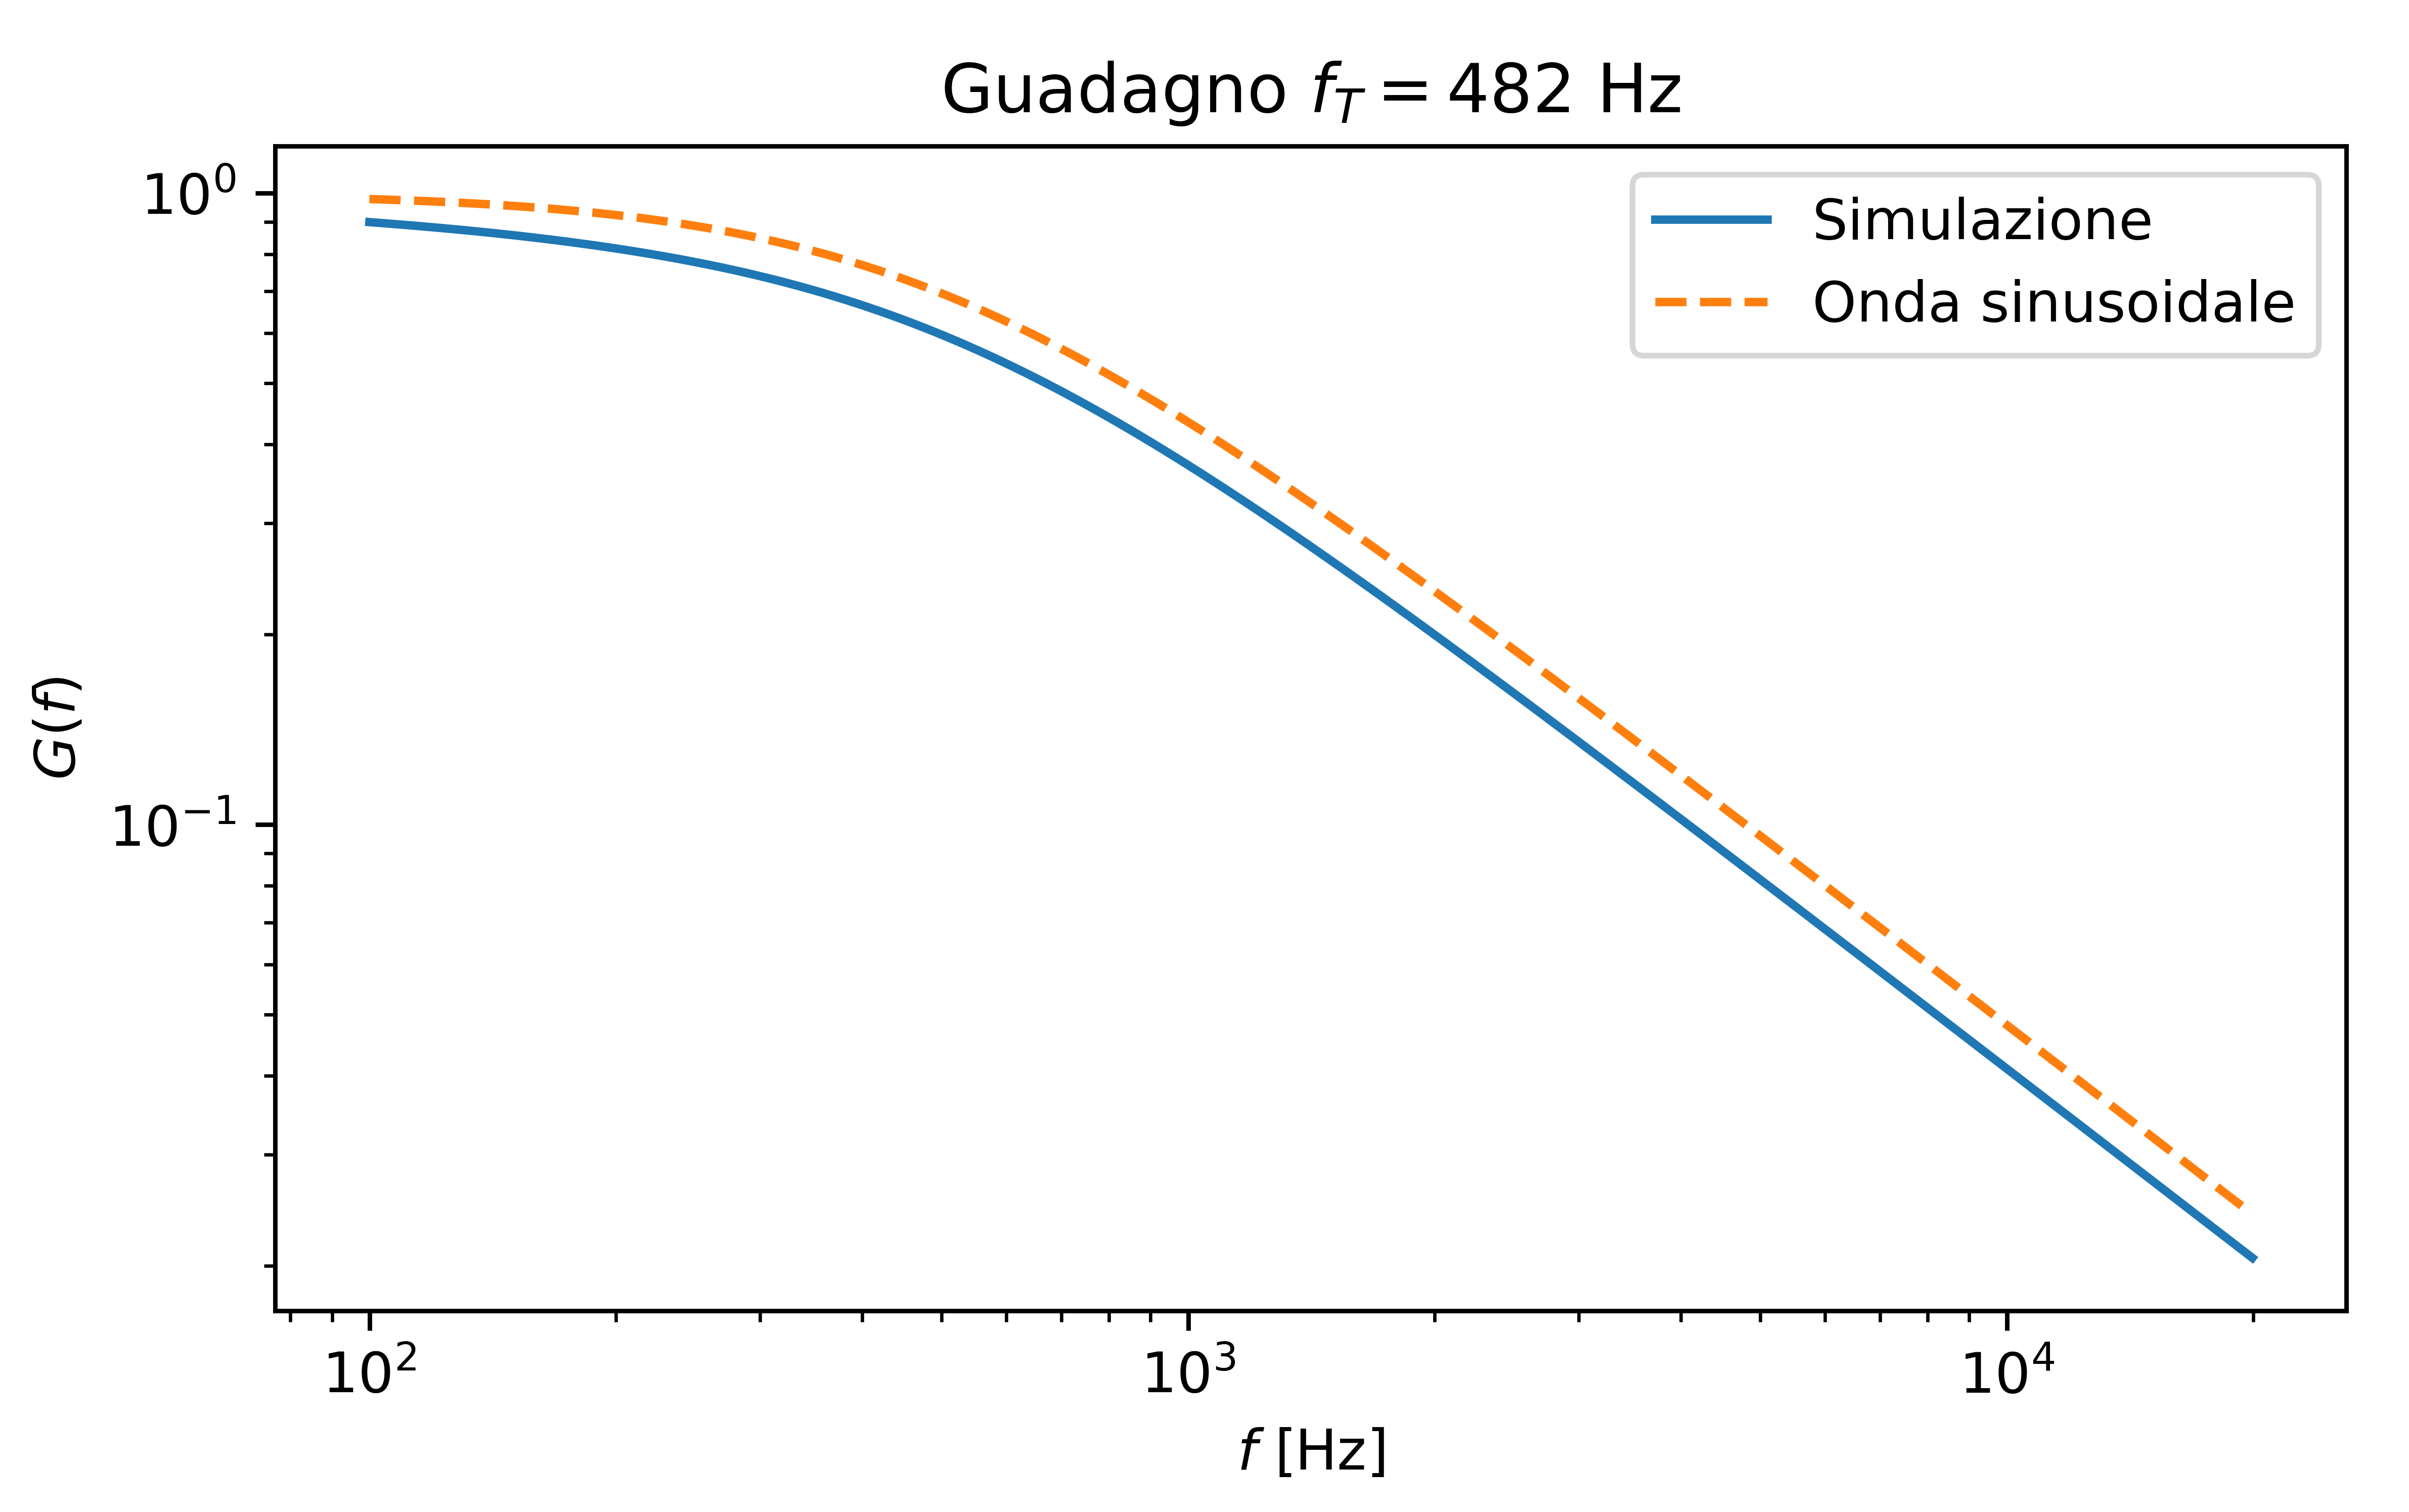
\includegraphics[width=0.9\textwidth]{img/Guadagno-T.png}
                \caption{Grafico guadagno $G(f)$ per $f_T=482$ Hz.}
            \end{figure}

\section{Ricostruzione onda quadra attraverso derivatore}
    Per un derivatore, guadagno e sfasamento sono dati da:
    \begin{align*}
        G(f) &= \frac{1}{\sqrt{1+(f_T/f)^2}}\\
        \Delta\phi(f) &= \arctan(f_T/f)
    \end{align*}
    Come per l'integratore, se mandiamo un'onda quadra attraverso un derivatore, l'onda in uscita avrà espansione in serie di Fourier data da (\ref{eq-pinna}), dove $G(f)$ e $\Delta\phi(f)$ sono come sopra.\\
    Abbiamo ricostruito numericamente gli andamenti in uscita a varie frequenze, lasciando la frequenza di taglio $f_T = 482$ Hz.\\
    Possiamo notare dai grafici che per $f<f_T$ l'onda consiste in spikes e risulta sfasata di un quarto di periodo a sinistra. Gli spikes sono dovuti al fatto che la derivata dell'onda quadra, matematicamente, sarebbe infinita nei punti di salto e nulla negli altri. Gli spikes hanno una coda a destra, mentre sono ripidi a sinistra. Questo è dovuto al fatto che il derivatore compie l'equivalente analogico di una derivata sinistra.\\ 
    Al crescere di $f$ i tratti orizzontali dell'onda assumono un andamento esponenziale, tipico della carica e scarica del condensatore. Per $f\gg f_T$ la forma d'onda tende a quella originaria.
    \begin{figure}[H]\label{fig:derivatore}
        \centering
        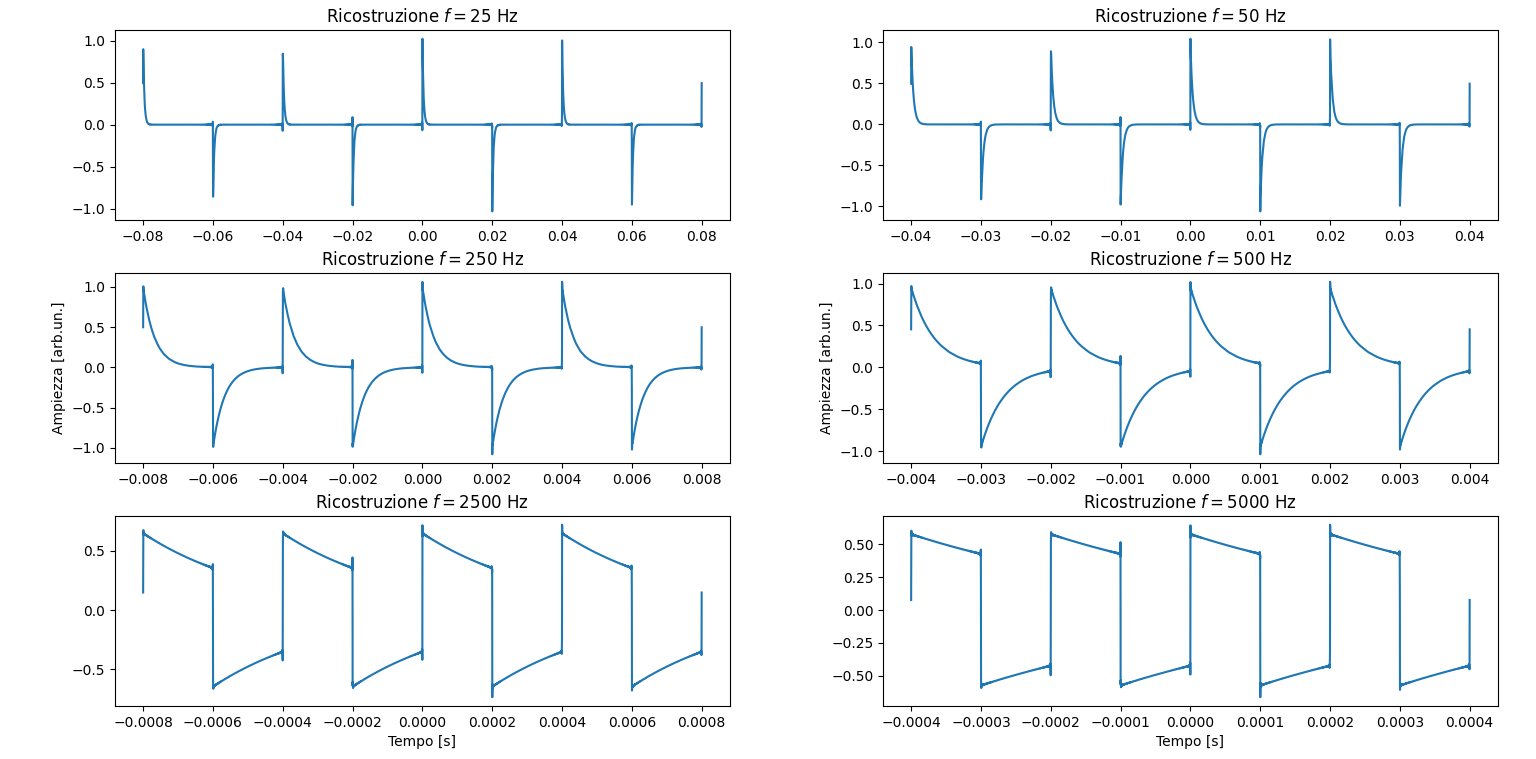
\includegraphics[width=1.0\textwidth]{img/Ricostruzione_spikes.png}
        \caption{Ricostruzioni al variare di f, per $f_T = 482$ Hz.}
    \end{figure}
    

\section{Ricostruzione numerica della d.d.p. in uscita da un livellatore con ingresso un treno di impulsi}
    In questa sezione, ricostruiamo il segnale in uscita da un livellatore con in ingresso un treno di impulsi con duty cycle variabile \textit{à la} modalità PWM di Arduino. Il segnale di ingresso può essere rappresentato dalla serie:
    \[g(t)=\delta+\sum_{k=1}^{n} \frac{2}{k\pi} \sin(k\pi\delta)\cos(\omega_kt)\]
    dove $\delta = \tau/T$ rappresenta il duty cycle, dato dal rapporto fra durata della parte alta dell'impulso $\tau$ e il periodo del treno di impulsi $T$.
    Applicando guadagno e sfasamento di un integratore alle componenti armoniche di $g(t)$ otteniamo il segnale in uscita dal livellatore.\\
    Per la ricostruzione numerica, abbiamo preso come $\tau$ caratteristico del livellatore 0.015 s (per una frequenza caratteristica di 66 Hz, valore prossimo a quello usato da noi in laboratorio, quando abbiamo effettuato l'esperimento con Arduino). Come frequenza del segnale abbiamo invece preso $f=1$ kHz.
    \begin{figure}[H]
        \centering
        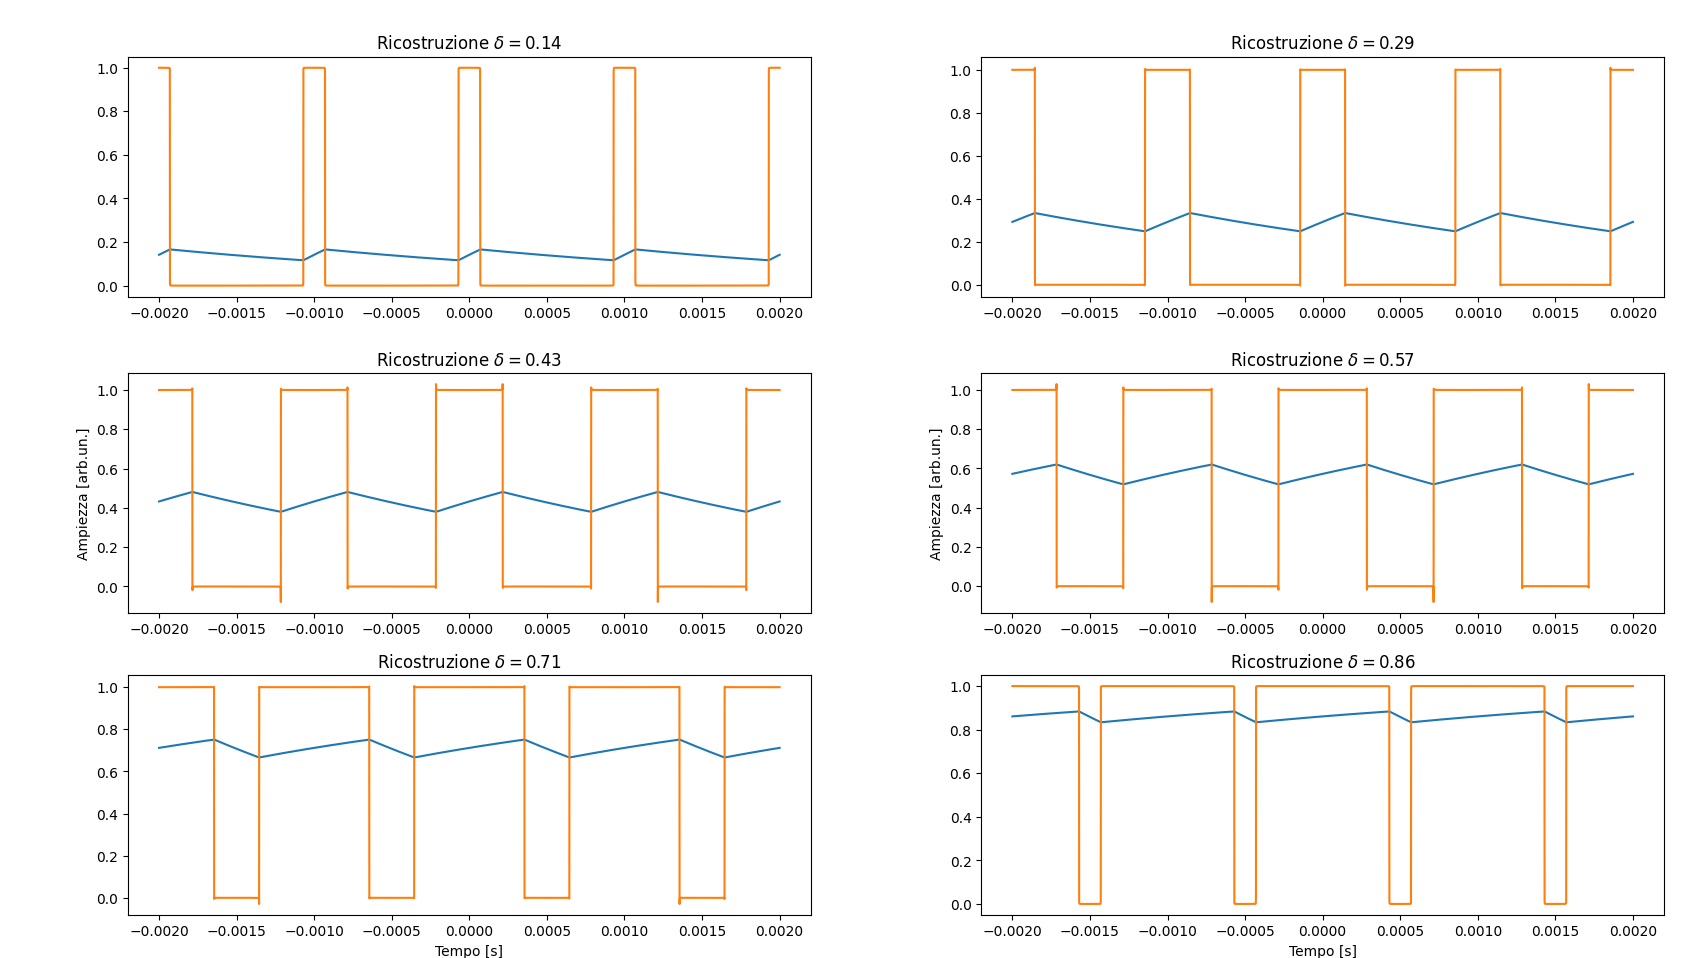
\includegraphics[width=1.0\textwidth]{img/PWM.png}
        \caption{Ricostruire numericamente la d.d.p. in uscita dal livellatore.}
    \end{figure}


\section{Ricostruzione forma d'onda quadra in accoppiamento AC}
    L'accoppiamento AC in ingresso all'oscilloscopio taglia la componente continua del segnale visualizzato, grazie alla presenza di un condensatore collegato in serie al segnale. Questo, una volta caricato, impedisce il passaggio di corrente, eliminando di conseguenza la parte continua del segnale. Assieme alla resistenza di ingresso dell'oscilloscopio ($R_{osc} = 1$ M$\Omega$), montata in parallelo al segnale, il condensatore realizza un circuito derivatore RC, ovvero un filtro passa-alto. Il segnale visualizzato sarà quindi come quelli in figura (\ref{fig:derivatore})
    Notiamo inoltre che l'ampiezza picco-picco visualizzata in AC è maggiore di quella effettiva della forma d'onda a causa dell'operazione di derivata temporale. 
    \begin{figure}[H]
        \centering
        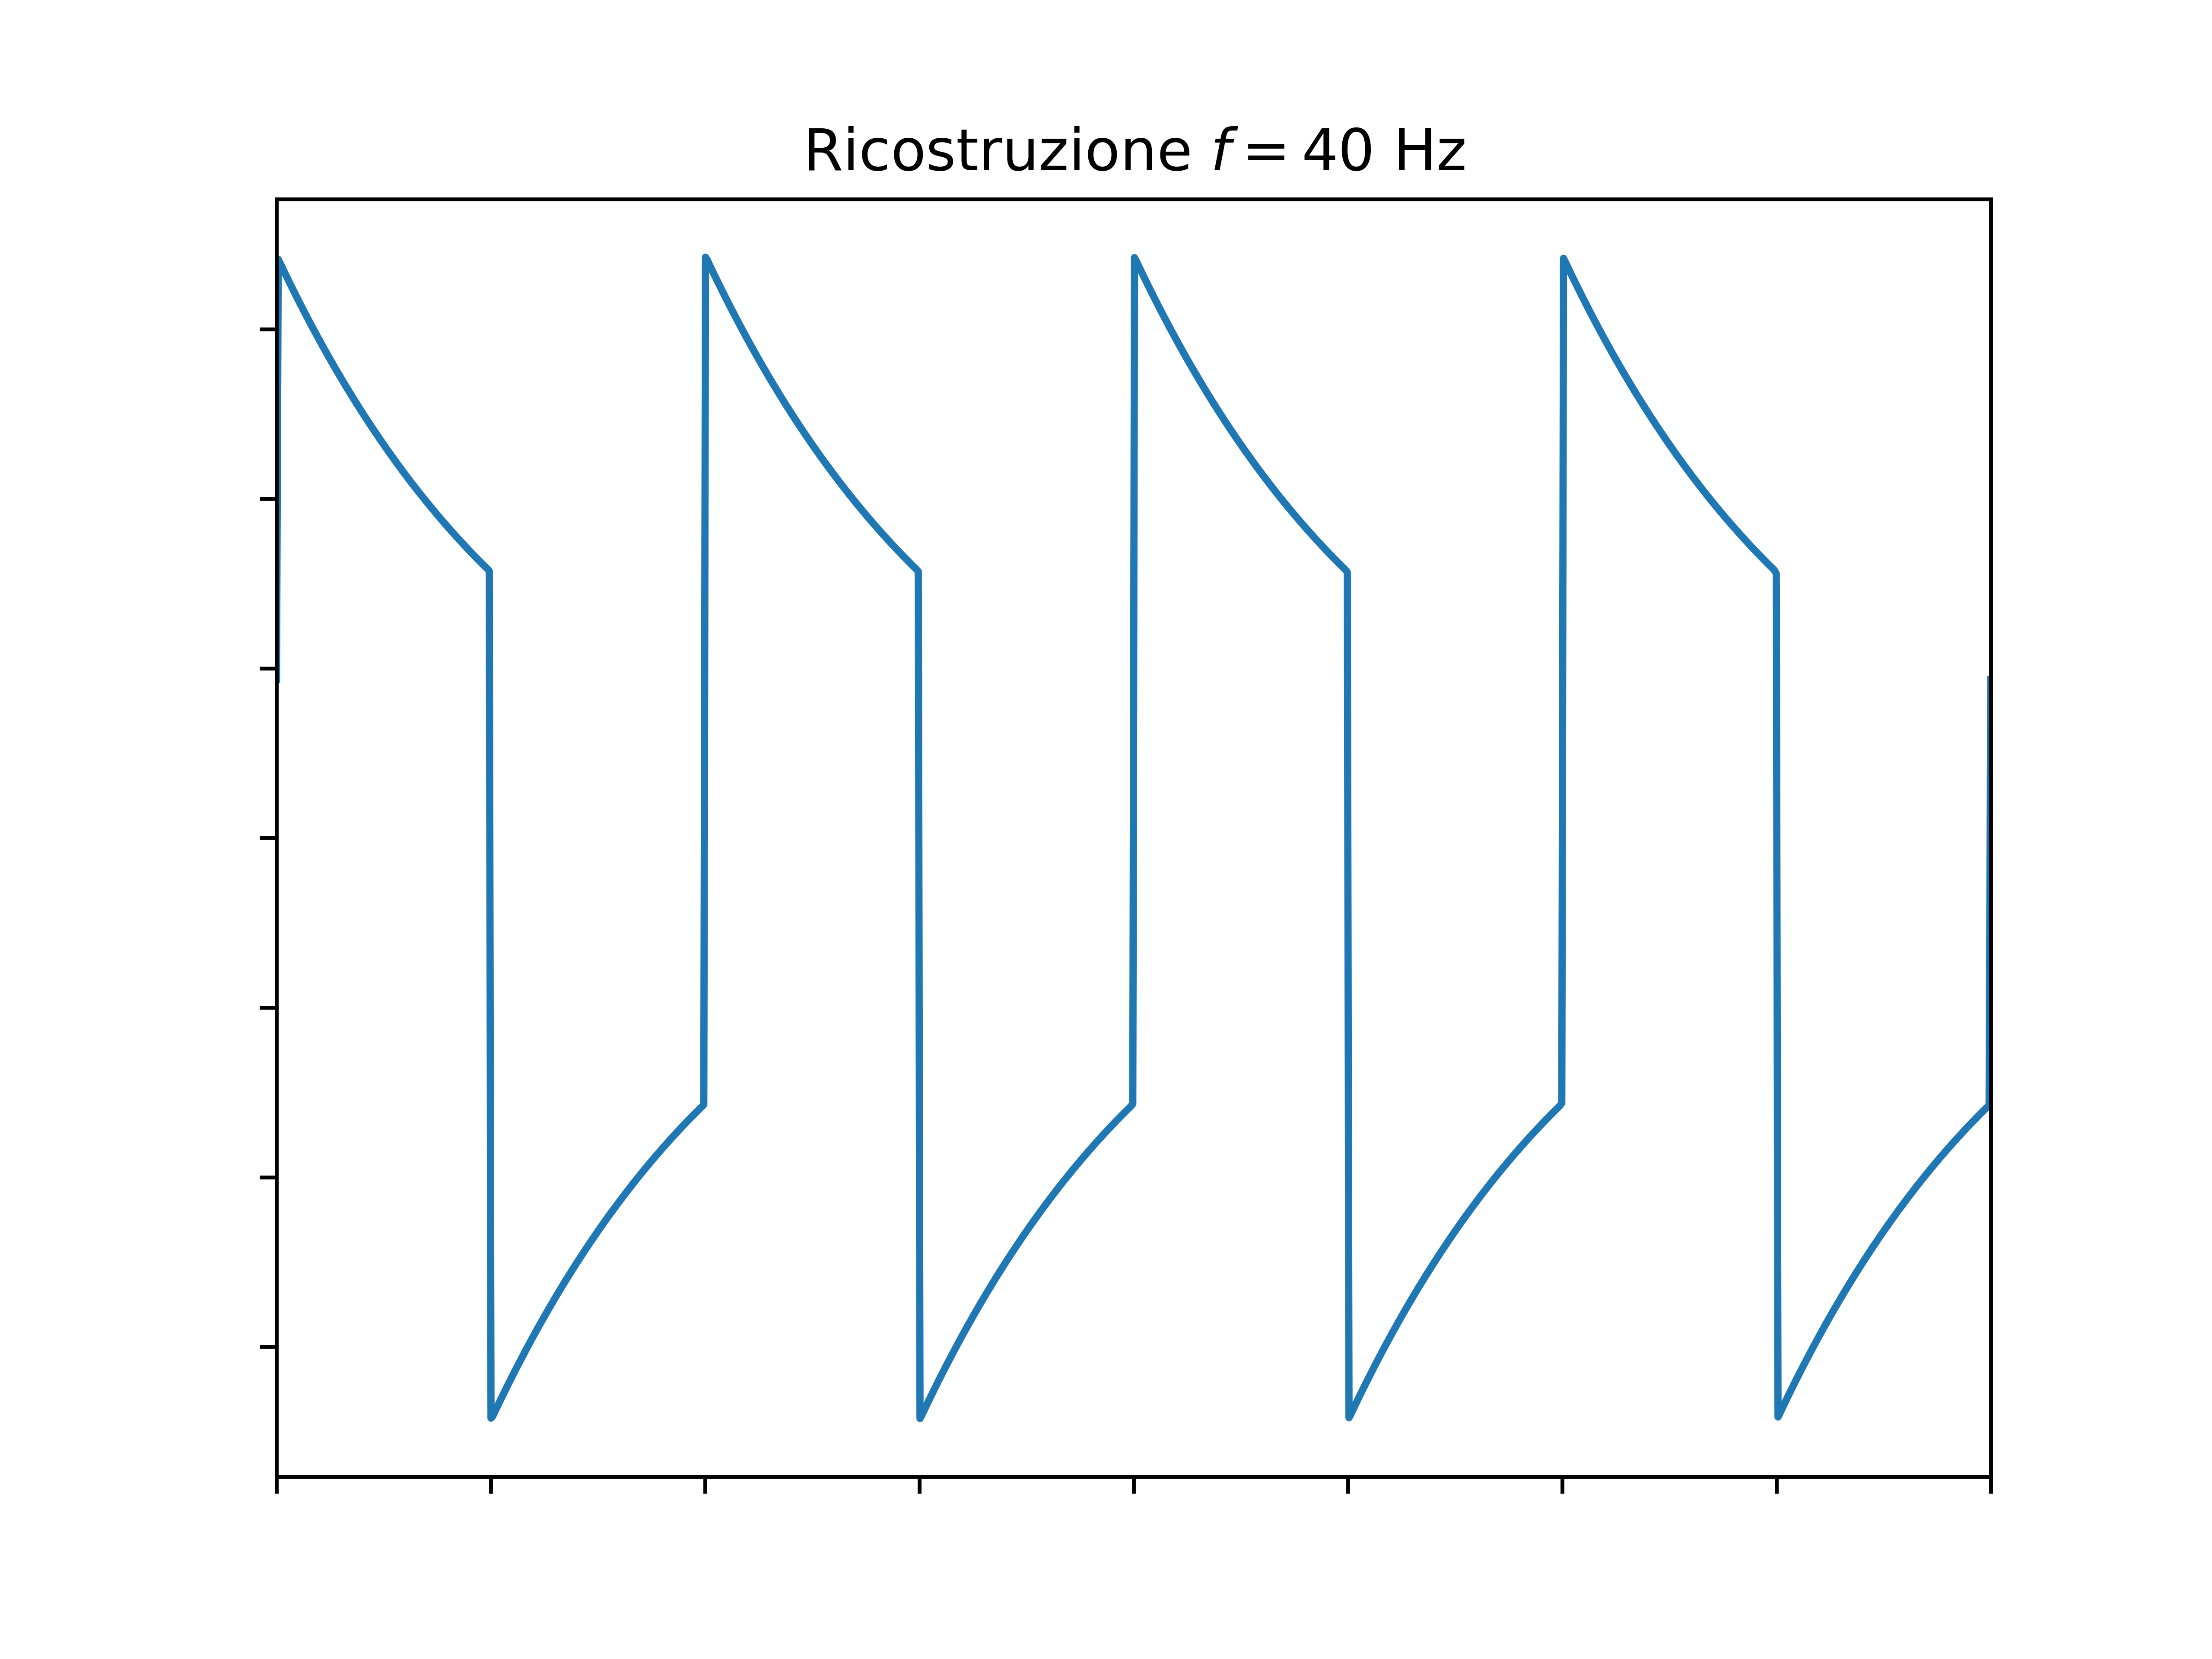
\includegraphics[width=0.80\textwidth]{img/Accoppiamento_AC.png}
        \caption{Simulazione della visualizzazione di un'onda quadra di frequenza $f = 40$ Hz con un oscilloscopio accoppiato in AC. Il derivatore in ingresso all'oscilloscopio è supposto avere $f_T = 10$ Hz.}
    \end{figure}

\section{Appendice: derivazione della correzione al guadagno $\Delta G$}
    \begin{figure}[H]
        \centering
        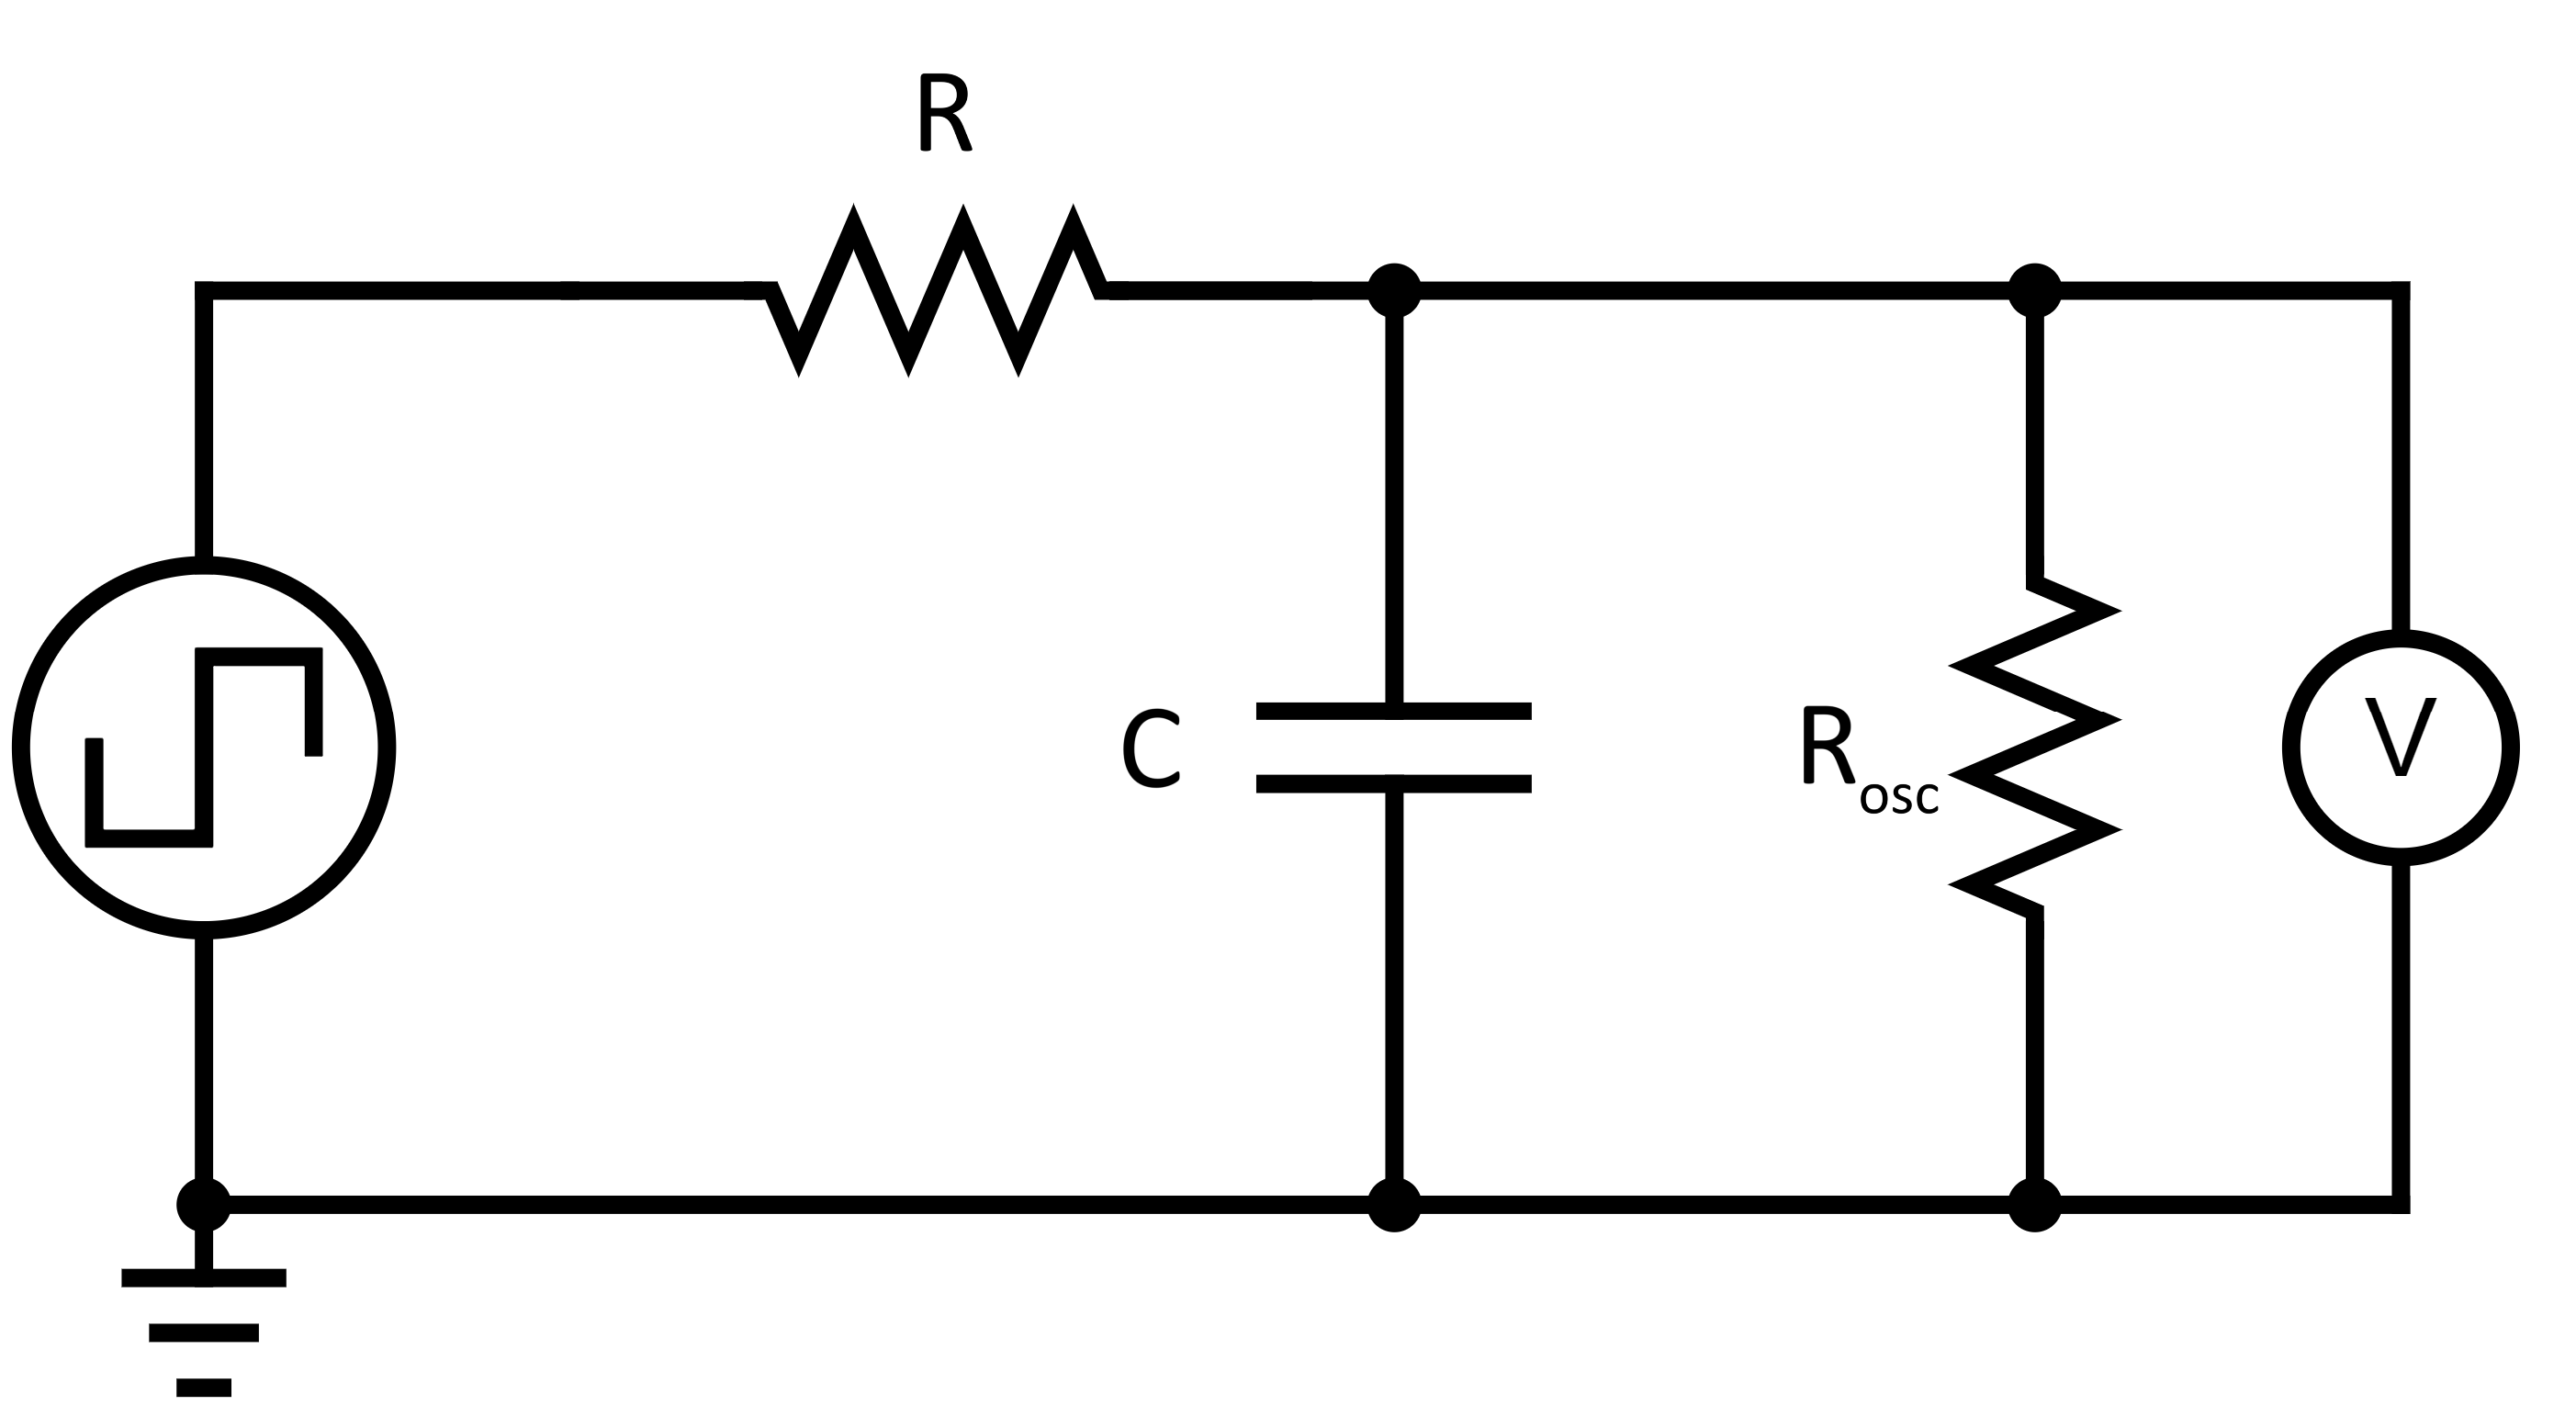
\includegraphics[width=0.45\textwidth]{img/circuito.png}
    \end{figure}
    Chiamando $R$ e $C$ rispettivamente la resistenza e la capacità del condensatore usati per l'integratore e $R_{osc}$ la resistenza interna dell'oscilloscopio, l'impedenza del circuito è pari a:
    \begin{align*} 
    Z &= R + \frac{1}{j\omega C + 1/R_{osc}} \\
    &\approx R + \frac{1}{j\omega C}\left(1-\frac{1}{j\omega R_{osc}C}\right)\\
    &= R + \frac{1}{\omega^2C^2R_{osc}} + \frac{1}{j\omega C}
    \end{align*}
    Dalle equazioni $V_{\omega, in} = Z I_{\omega}$ e $V_{\omega, in}-V_{\omega, out} = RI_{\omega}$, otteniamo l'espressione per la funzione di trasferimento:
    \[V_{\omega, in}-V_{\omega, out} = \frac{R}{Z} V_{\omega, in}\]
    \[T(\omega) = 1-\frac{R}{Z} = \frac{1+j\frac{1}{\omega R_{osc}C}}{1+j\frac{\omega}{\omega_T} + j\frac{1}{\omega R_{osc}C}}\]
    Introducendo per comodità la quantità $\Tilde{\omega}_T = \frac{1}{R_{osc}C}$, possiamo riscrivere quest'espressione come:
    \[T(\omega)=\frac{1 + j\frac{\Tilde{\omega}_T}{\omega}}{1 + j\frac{\omega}{\omega_T} + j\frac{\Tilde{\omega}_T}{\omega}}\]
    A questo punto, il guadagno $G$ è dato dal modulo di $T$:
    \[G(\omega)=\sqrt{\frac{1+(\Tilde{\omega}_T/\omega)^2}{1+ (\omega/\omega_T + \Tilde{\omega}_T/\omega)^2}}\]
    Poiché $\Tilde{\omega}_T\ll \omega,\omega_T$, espandiamo al primo ordine in $\Tilde{\omega}_T$:
    \begin{align*}
    G(\omega) &= \sqrt{\frac{1}{1+(\omega/\omega_T)^2 + 2\Tilde{\omega}_T/\omega_T}}\\
    &\approx \sqrt{\frac{1}{1+(\omega/\omega_T)^2}\left(1-2\frac{\Tilde{\omega}_T/\omega_T}{1+(\omega/\omega_T)^2}\right)}\\
    &\approx \sqrt{\frac{1}{1+(\omega/\omega_T)^2}} \left(1 - \frac{\Tilde{\omega}_T/\omega_T}{1+(\omega/\omega_T)^2}\right)
    \end{align*}
    Da quest'espressione leggiamo la correzione $\Delta G$:
    \begin{align*}
    |\Delta G(\omega)| &= \sqrt{\frac{1}{1+(\omega/\omega_T)^2}} \frac{\Tilde{\omega}_T}{\omega_T(1+(\omega/\omega_T)^2)}\\  
    &= \left(\frac{1}{1+(\omega/\omega_T)^2}\right)^{\frac{3}{2}} \frac{\Tilde{\omega}_T}{\omega_T}
    \end{align*}
    Scrivendo quest'espressione in termini della frequenza $f$ e della frequenza di taglio $f_T$ ed esplicitando $\Tilde{\omega}_T$, otteniamo l'espressione:
    \[|\Delta G(f)|= \left(\frac{1}{1+f^2/f_T^2}\right)^{\frac{3}{2}} \frac{1}{2\pi f_TR_{osc}C}\]
\end{document}
 